\documentclass[12pt,titlepage,a4paper]{article}
\usepackage{graphicx}
\graphicspath{{images/}}


\usepackage[ngerman]{babel}
\usepackage[utf8]{inputenc}
\usepackage{color}
\usepackage[a4paper,lmargin={2cm},rmargin={2cm},
tmargin={2.5cm},bmargin = {2.5cm}]{geometry}
\usepackage{amssymb}
\usepackage{amsthm}

%\usepackage{cite}
\usepackage{natbib}
\usepackage{blindtext}
\usepackage{enumitem}
\usepackage[toc]{glossaries}
%\setlist[description]{leftmargin=\parindent, labelindent=\parindent}
\usepackage{wrapfig}
\usepackage{listings}

\makeglossaries
\newglossaryentry{cpu}
{
name = CPU,
description = {\textit{Central processing unit}, alias Prozessor, erledigt die meisten Aufgaben eines Computer bei der es um die Berechnung von Werten geht.}
}

\newglossaryentry{Transistor}
{
name = Transistor,
description = {Elektronisches Bauteil mit 3 Pins. Wird gebraucht, um Stromflüsse zu kontrollieren und zu verstärken.}}













%Dokument beginnt
\begin{document}
%Titlepage
\begin{titlepage}
\title{Smart Growbox}
\date{2020}
\author{Jonas Valentin Rose}
\end{titlepage}
\maketitle 
\tableofcontents
\newpage
% Ab jetzt Fliesstext
\section{Einleitung}
Dies ist der schriftliche Teil meiner Maturarbeit, bei welcher ich mich  mit der Konstruktion einer möglichst schlauen Growbox auseinandersetze. Ich stelle hier so viel möglich und so wenig wie nötig alle meine Gedanken vor, welche mich während dieser Zeit motivierten oder plagten. Angefangen bei der Idee selbst, über die pflanzlichen Anforderungen, weiter zu den drei Kernelementen des Konstrukts bis hin zum esten Webserver und einer Dämonenbeschwörung. Ich möchte Ihnen einen möglichst nahen Einblick in meine letzten paar Monate zu geben.


\subsection{Idee}
Mögen Sie Tomaten? Ich tue es, im Sommer 2019 habe ich meine eigenen gezüchtet, direkt auf meinem Balkon. Sie stellten sich als recht gut gereift heraus. Allerdings plagte es mich, während des vierwöchigen Korsika-Urlaubs die Verantwortung bezüglich der Bewässerung abzugeben. Nicht dass ich gerne selbst Pflanzen bewässere, klar es hat durchaus etwas magisches an sich. Faul lässt es sich am besten clever leben, ergo: Es muss eine richtige Lösung her, eine Automatische. Ich möchte in den Urlaub fahren können, ohne die Verantwortung meiner Stecklinge abgeben zu müssen, aber ich möchte mir auch nicht die ganze Zeit Sorgen machen müssen. Ich will den \textit{Föifer} und \textit{s'Weggli}. Meine Tomaten sollen wachsen, aber ohne meine Bemühungen. Eine Maschine muss her! Eine solche, mit der man dem Tomätchen die perfekten Wachstumsbedingunen geben kann, ohne sich auch nur darum zu bemühen. \\ Das mit der Bemühung ist so ein Thema, denn zuerst will die Maschine gebaut sein. Ich stelle sie mir so vor: Eine Growbox in meinem Zimmer mit künstlicher Beleuchtung, automatischer Bewässerung und einem sich selbstregulierenden Belüftungssystem. Klingt gewagt, aber nicht unmachbar. Ich beweise es Ihnen.

\subsection{Ziel und Abgrenzung}
\subsubsection{Das Konstrukt}
Im praktischen Teil konstruiere ich eine Maschine, welche mir Esspflanzen züchtet. Sie soll die drei Hauptaufgaben übernehmen, welche ich als Belüftung, Beleuchtung und Bewässerung identifiziert habe. Sie soll selbst gebaut sein, d.h. keine fremde Regelungstechnik wie Zeitstromschalter oder Thermostaten. Die Finanzierung erfolgt selbst. Ich werde die Bauteile selbst kaufen/zusammenbauen/konstruieren/programmieren und das dazugehörige Wissen beziehe ich grösstenteils aus dem Internet. Ich mache auch von der Erfahrung meines Vaters gebrauch, er steht mir in besonders abstrakten Problemstellungen bei.
\subsubsection{Schriftlicher Teil}
Hier im schriftlichen Teil gebe ich dem Leser einen möglichst direkten Einblick in die Lösungsfindung der Teilprojekte. Was ich nicht vorhabe, ist Python, C++ oder Löten zu erklären. Sie werden hin und wieder auf Codesnippets treffen. Aus diesen Gründen ist es von Vorteil, wenn Sie schon etwas mit Technik zu tun haben. Nebst dem Arbeitsprozess schildere ich im nächsten Kapitel auch meine Motivation, dieses Projekt nicht \textit{nur} als Maturarbeit zu verfolgen. Anschliessend werde ich mit möglichst wenigen aber klaren Sätzen das \textit{Konstrukt} selbst erklären, wie es funktioniert, wo die Tücken liegen und worauf ich besonders Stolz bin. Im Kapitel \textit{Perspektiven} gehe ich auf alles ein, was mich rund um die Arbeit beschäftigte. Zu guter Letzt ziehe ich ein Fazit und bedanke mich bei allen Menschen, welche mir geholfen haben, mein Vorhaben in die Realität umzusetzen.

\newpage
\section{Motivation}
Ich verbringe (zu) viel Zeit auf YouTube\footnote{$https://www.youtube.com/$}. Eine mich inspirierende Gattung sind die Art Videos, welche sich mit Offgrid-Versorgungssystemen beschäftigen, also der Nahrungs-/Energieversorgung eines Lebensraums ohne Teil des Hauptnahrungs-/energienetzes zu sein. Dieses \textit{Autarksein} fasziniert mich. Des Weiteren stiess ich vor etwa 10 Monaten auf den Kanal von \textit{Jeb Gardener}\footnote{$https://www.youtube.com/channel/UC5zdi4KM3ewwfYMNo_KnU0A$}. Ich fasse die Gemeinsamkeiten seiner Videos mit folgendem Satz zusammen: Verrückter Gärtner züchtet mit komplett unkonventionellen und (laut einigen Stimmen aud dem \textit{traditionellen Gärtnermilieu}) ethisch kritischen Methoden Pflanzen. Seine Bewässerungsmethoden sind überaus selten traditioneller Art, bedeutet, dass er fast immer auf Erde verzichtet. Er stellt die Pflanzen direkt ins Wasser. Beleuchtet wird künstlich, mit pinken LEDs und die Nährstoffe sind synthetisiert und werden einfach ins Wasser geworfen, wo sie sich auflösen. Konventionalität interessiert ihn nicht. Dazu kommt noch, und das ist fast das Beste, dass seine Videos durch die musikalische Begleitung von epischer Orchestermusik eine fast zerreissende Spannung erreichen. Stellen Sie sich einen \textit{durchgeknallten} Gärtner vor, der von einem Streichorchester begleitet Wurzeln filmt. Seine Unverdrossenheit im Umgang mit Anbaumethoden ist sehr ansteckend. \textit{Whatever gets the job done.} \\ Segelvideos sind auf YouTube seit ein paar Jahren ebenfalls sehr \textit{in}, sie verdanken ihren Erfolg wohl dem Freiheitstraum vieler \textit{Landratten}. Der YouTube-Zuschauer sieht durch seinen Bildschirm den den Sonnenuntergang im unendlichen Horizont und versucht sich den Wind in den Haaren vorzustellen. Der Segler lebt diesen Moment und fängt es mit der Kamera ein. Es ist ein Zusammenspiel und ich bin ein Teil davon. Was aber hat das mit meiner Maturarbeit zu tun? Hier der Link: Bei einer Ozeanüberquerung hat man nach ein paar Wochen keine frischen Lebensmittel mehr, die Rede ist von Früchten, frischen Kräutern und Gemüse. Was aber, wenn man sich seine Lieblingstomaten einfach selbst auf dem Boot züchtet? In einer Miniaturversion meines Konstrukts, mit Solarpanels als Energieversorgung. Wäre das nicht einfach genial? Ich könnte Do-It-Yourself-Anleitungen machen, sodass mehr Segler \textit{mehr} frische Sachen essen können. Durch \textit{Der verschenkte Sieg}\footnote{B. Moitessier, ISBN 978-3-7688-0749-4, Gedruckt 2008 in Deutschland, Delius Klasing Verlag, Original: \textit{La longue route}} von \textit{Bernard Moitessier} habe ich gelernt, wie sehr frisches Gemüse oder Früchte die Lebensqualität auf einer Pazifiküberquerung heben können. Die oben genannten Erkenntnisse motivieren mich, das \textit{Konstrukt} nicht nur als Maturprojekt sondern als Lebensprojekt zu verfolgen.
\newpage







\section{An die Arbeit}
\subsection{Wachstumsbedingungen}
Das Hauptziel in dieser Arbeit ist die Zucht von Pflanzen durch eine künstliche Umgebung. Pflanzen haben Ansprüche und um die geht es jetzt kurz. Mit einer für die Arbeit tragbaren Tiefe erkläre ich warum sie bestehen.

\subsubsection{Wasser}
Pflanzen brauchen Wasser für den Transport von Nährstoffen, für die Photosynthese und um den Zelldruck und die damit verbundene Stabilität zu erhalten - unbewässerte Pflanzen lassen bekanntlich ihre Köpfchen hängen.


\subsubsection{Licht}
Licht ist die Energieform, welche sich die Pflanze bei der Photosynthese zunutze macht, um energiearme Baustoffe in Energiereiche zu verwandeln. Diese werden für den Bau und die Energiespeicherung verwendet. 

\subsubsection{Luft}
Luft, auch wenn eigentlich überall vorhanden, muss einen genügend grossen CO$_{2}$-Anteil enthalten, um der Pflanze die Photosynthese zu ermöglichen. Sie wird, wie das Licht grösstenteils, über die Blätter aufgenommen.

\subsubsection{Nährstoffe}
Nebst der selbst hergestellten Glucose verwendet die Pflanze auch noch andere Bausteine um sich Struktur zu geben und um den Stoffwechsel zu betreiben. Diese können nicht aus der Luft gefischt werden, sondern werden in gelöster Form von den Wurzeln aufgenommen. Dazu zählen Elemente wie Phosphor, Kalium und Stickstoff.\footnote{Selbsverständlich gibt es mehr, die genannte werden zu den \textit{Makronährstoffen} gezählt. $https://www.thespruce.com/what-are-plant-macronutrients-1902843$}

\clearpage
\subsection{Wie weiter?}
Ich kenne nun die Ansprüche meiner Pflanzen, aber wie baue ich eine Maschine, die diesen entgegen kommt? Dies ist der Kern der Arbeit. In diesem Kapitel stelle ich vor, wie ich mir die Konstruktion vorstelle und wie ich an die verschiedenen Herausforderungen herangegangen bin.\\ Zuerst benötige ich Bauteile, doch von wo nu- Ach ja genau, das Internet, es ist voll mit Möglichkeiten, Produkten und Wissen.
Materialsuche ist ein anstrengendes Unterfangen, ich bin aber nochmal glimpflich davongekommen, denn ich fand  eine gute Menge Material in der Kellerwerkstatt meines Vaters. Er ist ein \textit{Techie}, der gerne Elektroteile sammelt, zu meinem Glück.

\subsection{Baumarkt, Cannabis-Shops und der Keller}
Hier sind die essenziellen Bauteile des \textit{Konstrukts}.
\begin{description}
\item[Growbox] Die Schale stellt meine Growbox\footnote{$https://www.growshop.ch/growbox-secret-jardin-dark-room-r3-dr60.html$} dar, sie besteht aus einem Plastikgewebe, das an der Innenseite mit Mylar\footnote{$https://en.wikipedia.org/wiki/BoPET$} beschichtet ist - es reflektiert zu einem hohen Bestandteil Licht. Sie bietet Schutz und ermöglicht es den Pflanzen, ein eigenes Klima zu entwickeln, eine eigene, kleine Ökosphäre sozusagen.
\item[LEDs] Ich beleuchte meine Pflanzen künstlich mit zwei 50 Watt LEDs\footnote{$https://www.growlight.ch/$}. Beide sind auf die für die Pflanze essenziellen Lichtspektren eingestellt, was sich für das menschliche Auge als ein pinkes Helligkeitswunder herausstellt. Es schmerzt, ich hätte besser nicht reingeschaut..
\item[Fogger] Ein Wundergerät\footnote{$https://www.visionofhemp.ch/shop5/en/$}, es macht aus flüssigem Wasser einen Nebel. Damit kann ich die Wurzeln über die Luft mit Wasser und Nährstoffen versorgen, mehr dazu gleich.
\item[Wasserbecken] \textit{Baumarkt} hat ein beachtliches Sortiment an \textit{Zementmischeimern}, einen davon habe ich erworben.
\item[Sensoren] Um zu wissen, wie fest ich Lüften muss, brauche ich Sensoren. Zu meinem Erfreunis sind sie äusserst günstig.
\item[Microcontroller] Die meisten Microcontroller, namentlich Arduinos\footnote{$https://www.arduino.cc/$} und einen RaspberryPi\footnote{$https://www.raspberrypi.org/$} hatte ich dank meinem \textit{Geekvater} schon zuhause.
\item[Sonstige Elektronik] Kleinere Bauteile für die verschiedenen Schaltungen hat ebenfalls die Kellerwerkstatt meines Vaters beigesteuert. Darunter befinden sich vor allem Drähte, Kabel, Widerstände, Transistoren und Dioden.
\item[Lüfter] Aus der edlen CPU-Lüftersammlung meines Vaters konnte ich vier Gleichstrom-Lüfter ergattern.
\item[Pflanze] Das ganze Projekt würde ohne Pflanzen nicht funktionieren. Beim \textit{Gartenmeier Center}\footnote{$https://www.meier-ag.ch/$} beschenkte ich mich mit Tomatenstecklingen, zweimal, denn das Projekt hat länger gedauert als angenommen, wodurch der erste Satz Stecklinge leider dran glauben musste.
\item[Nährstofflösung/Dünger] Mit einer Universalnährstofflösung vom \textit{Gartenmeier Center}(die sogar den richtigen pH-Wert mit sich bringt) kann ich nichts falsch machen. Auch darauf komme ich nochmal zu sprechen.
\end{description}

\subsection{Trockenes Wasser}
Durch\textit{ Jeb Gardner} wusste ich von der Hydroponik\footnote{$https://en.wikipedia.org/wiki/Hydroponics$} schon vorher und durch Zufall stiess ich auf Fogponik\footnote{$https://en.wikipedia.org/wiki/Fogponics$}, was sich als recht eleganten Ansatz herausstellt. Man zählt Fog-, respektive Aeroponi\footnote{$https://en.wikipedia.org/wiki/Aeroponics$} als eine Unterkategorie der Hydroponik. Konkret geht es dabei um die Bewässerung der Pflanze, während sich ihre Wurzeln \textit{in der Luft befinden}, also weder im Wasser, noch in einem Substrat. Düsen werden gerne in grossen, industriellen Gewächshäusern verwendet, doch nach endloser Recherche musste ich mir eingestehen, dass Düsen einfach sehr schwer zu bestellen sind. Ich erweiterte also meinen Horzizont. Fogponics sind genial, man nimmt den Fogger (ein recht schweres, wasserfestes Metalding mit fünf Porzellanscheiben), setzt ihn ins Wasser und schaltet ein. Die Porzellanscheiben vibrieren mit 1.7MHz, also etwa etwa alle 0.6 Microsekunden einmal, und spicken somit feinste Wassertröpchen in die Luft - Ein Nebel entsteht. Wenn im Wasser dann noch die essentiellen Nährstoffe gelöst sind, hat man einen Nährstoffnebel! Die Tröpfchen sind ca. ein \textit{Zweihundertstelmillimeter}, was es ihnen ermöglicht, direkt in die Wurzeln einzudringen, ohne dabei an der Wurzelwand zu kondensieren. Eine so direkte Nährstoffaufnahme ist \textit{giga-effizient} und nur bei solch kleinen Tröpfchen möglich.  \\ 
Kleiner Seitenfakt: Beim Einatmen von solch kleinen Tröpfchen muss man Husten, denn sie ähneln mehr einer Art Staub als Wasser. Das ist wahrscheinlich auf ihre eingeschränkte Kondensfähigkeit zurückzuführen, was sie für uns \textit{nass} machen würde. Diese Technologie wurde unter anderem durch die Nasa erforscht\footnote{$https://aeroponicsdiy.com/nasa-review-of-aeroponics/$}. Ich verwende es nun, um Pflanzen \textit{intrawurzulös} mit trockenem Wasser und Nährstoffen zu versorgen, auch gut.

\subsection{Belüftung..}
Die Lüfter waren ebenfalls ein lustiges (\textit{trockenes, kaltes Lachen}) Teilprojekt: Um ein Lüftungs-system zu bauen, benötigt man offensichtlich einen Lüfter, am besten gleich mehrere. Es gilt zwischen EC- und DC-Lüftern zu unterscheiden, wobei EC-Lüfter generell leiser und energieeffizienter sind. Naheliegenderweise hätte ich gerne einen Lüfter der EC-Gattung, doch da mein Vater ein leidenschaftlicher Sammler jeglichen Elektroschrotts ist, konnte ich mich einfach im Keller bedienen. Um es kurz zu fassen: Bei der Belüftungskonstruktion habe ich meine Seele verloren, es ist das Teilprojekt mit dem meisten Aufwand. Das mit der Seele ist sinnbildlich gemeint Im Nachhinein habe ich mich wirklich gefragt, ob es dieser Aufwand nicht die 120Fr. wert gewesen wäre, was so ein EC-Lüfterchen kostet. Ich erläutere mal das Problem: Einen DC-Lüfter (Gleichstrom) runterzuregeln, so dass er nicht volle Pulle lüftet, ist eine Wissenschaft für sich, ich habe viel gelernt, doch zu welchem Preis? Einfach die Spannung runterzudrehen geht nicht wirklich, denn sie ist zwar proportional zur Umdrehungszahl, doch unter einem gewissen Wert springt der Lüfter gar nicht erst an. Was bleibt mir also? Ganz einfach - \textit{Pulsweitenmodulation}\footnote{$https://en.wikipedia.org/wiki/Pulse-width_modulation$}. 
Hier das Prinzip: Man versorgt den Lüfter entweder mit 12V oder mit 0V, aus dem zeitlichen Verhältnis zwischen diesen beiden Zuständen erfolgt die effektive Lüfterleistung. Ist der \textit{Puls} also 75\% eines gesamten Zyklus, läuft der Lüfter auch mit 75\%, klingt einfach, ist es aber nicht. Die Krux liegt in der Frequenz dieser Zyklen, es macht nämlich einen Unterschied, ob man ihn für 7.5s mit 12V versorgt und dann 2.5s Pause macht oder ob diese Zyklen mit einer Frequenz von 40'000Hertz aufgetischt werden. Beim ersten Beispiel stockt der Lüfter und beim Zweiten wird der Saft so unglaublich schnell an und abgestellt, dass der Motor gar nicht mehr zwischen An und Aus unterscheiden kann. Voilà, Pulweitenmodulation. \\ Die Theorie ist vergleichbar einfach, denn hier kommt die technische Umsetzung: Die von mir verwendeten Microcontroller besitzen eine vorprogrammierte PWM-Funktion, jedoch hat diese eine Maximalfrequenz von 1kHz, also 1000Hertz und das ist zu langsam, denn damit \textit{kann} der DC-Motor noch zwischen An und Aus unterscheiden und es kommt zu hörbaren Vibrationen. 
Das schlägt einem nach 2min recht auf den Wecker. Es muss demnach eine andere Lösung her. Der Arduino (der Microcontroller) ist rein technisch gesehen dafür ausgerüstet, höhere Frequenzen zu takten, ein gutes Beispiel dafür ist der Prozessor, der, wenn er auf 1kHz laufen würde, \textit{schnarchend} langsam wäre. Dem ist natürlich nicht so. Und auch wenn der eingebaute ATmega32U4
\footnote{$https://www.mouser.ch/datasheet/2/268/Atmel-7766-8-bit-AVR-ATmega16U4-32U4_Datasheet-1315135.pdf$}
Prozessor mit seinen 16MHz das weitaus schnellste Glied auf der Platine ist, weilen die internen Timer-Register nicht viel hinten. Die C++-Bibliothek \textit{TimerOne.h}\footnote{$https://playground.arduino.cc/Code/Timer1/$} beherbergt die nötigen Werkzeuge. Man kann sich einen eigenen Timer stellen, sagen wir auf 25 Mikrosekunden, und wenn immer dieser Timer abläuft, schalten wir entweder an oder aus. So ungefähr lautet das Prinzip, effektiv existiert aber schon eine eigens dafür entwickelte Funktion. Man muss nur den Pin angeben, die Frequenz vorher eingestellt haben und sagen, welches Verhältnis man wünscht. Perfekt für meine Ansprüche. \\
Soviel zum Softwareteil, der Hardwareteil ist auch eine rechte Herausforderung. Ich brauche für jeweils vier Lüfter eine Schaltung, welche den Strom auf einer so hohen Frequenz an- und ausschalten kann. Also gut, Platine her, Lötkolben und Oszilloskop raus und runter in die Werkstatt. Ich habe für diese Schaltung etwa einen Monat gebraucht, natürlich war ich nicht jeden Abend dran, doch die alleinige Dauer, welche ich vor dem Oszilloskop verbracht habe, um die richtigen Verhältnisse zu sehen, hat mir die Seele wahrlich etwas betäubt. Im Kapitel \textit{Perspektiven} gehe ich näher auf Gelerntes ein, deshalb verrate ich hier einfach, dass am Ende der sogenannte \textit{PWM-Controller} geboren war. Wie er funktioniert, erfahren Sie im Kapitel \textit{Technische Hintergründe}

\subsection{Es soll hell sein}
Die Belichtung ist simpler. Nichtsdestotrotz muss ich kurz ausholen:\\ Um sowohl die Belichtung, als auch die Bewässerung zu steuern, benötigt es einer weiterer Schaltung: Und zwar eine, die mal an und mal aus geht - und das bitte in einem von mir vorgegebenen Takt. Swoosh, geboren ist der \textit{Relay-Controller}! Auf den Bauprozess und die Funktion dieses Babys wird später eingegangen. Sie sollen einfach wissen, dass es recht gut funktioniert. Die Belichtung ist echt keine Hexerei, die LEDs gehören einfach eingesteckt und der Relay-Controller vorprogrammiert und es läuft. \\ Ein solcher LED-Schweinwerfer kostet 65Fr und ist rein von der Leistung gesehen (50W) für meine zu belichtende Grundfläche von 0.36m$^{2}$ hell genug. Warum habe ich also zwei davon? Erstens sehen diese LEDs total schön aus - sie haben auch so ein cooles Gehäuse, sollten Sie mal sehen, und andererseits hat mich - ob relevant oder nicht - die Frage beschäftigt, wie lang diese Babies denn so halten. Das Internet gibt keine genaue Angabe, deshalb habe ich mir, so genial wie ich bin, überlegt, dass ich, wenn ich den Arbeitsaufwand auf zwei verschiedene Lampen aufteile, die Haltbarkeit von diesem Teil der Maschine wohl doppelt so hoch sein muss. Und falls eine den Geist aufgibt, habe ich Ersatz da. Ich habe in der Einleitung schon von Sorgenfreiheit gesprochen, Ersatzteile sind ein Aspekt davon. Wer jetzt denkt, dass ich einfach beide einschalten kann, um meine Pflanzen zu boosten, muss ich leider enttäuschen, so einfach funktioniert die Biologie nicht, mehr dazu in \textit{Technische Hintergründe}.

\subsection{Das Hirn!}
Irgendjemand, oder besser gesagt irgend\textit{was} muss diesen gutmütigen Controllern eine Richtung weisen, ihnen sagen, was sie zu tun haben. An diesem Punkt würde ich mich gerne bei Herrn Upton\footnote{dem ursprünglichen Entwickler und heutigem CEO der Raspberry Pi Foundation $https://en.wikipedia.org/wiki/Eben_Upton$}, dem Gründer der RaspberryPi-Foundation bedanken, ohne ihn wäre dieses ganze Vorhaben nämlich recht \textit{hirnlos}, im wahrsten Sinne des Wortes: Ich verwende einen Raspberry Pi 4 als Zentrum für alle Steuerprozesse. Der Raspberry Pi \footnote{umgangssprachlich auch \textit{Pi}} beherbergt alle Funktionen welche man von einem normalen Computer erwarten würde, nur kleiner, denn er passt problemlos in die Hosentasche. Die Leistung ist geringer als bei Computer mit normalen Dimensionen, doch Rechenleistung steht bei vielen Projekten erst an zweiter Stelle. Ich z.B. brauche einfach einen anständigen Kernel und genau das liefert der Pi. Mit Linux bin ich gleichermassen aufgewachsen wie mit einem Fahrrad, es war halt da. Deshalb ist es mir eine Freude, dieses Schätzchen auf meine Bedürfnisse anzupassen. Da es in diesem Kapitel generell nur um die erste Herangehensweise geht, fasse ich mich kurz, denn der Pi kommt zeitlich erst recht am Schluss ins Projekt: Er steuert die Sachen, welche andere Sachen steuern und nimmt Inputs vom Benutzer entgegen.

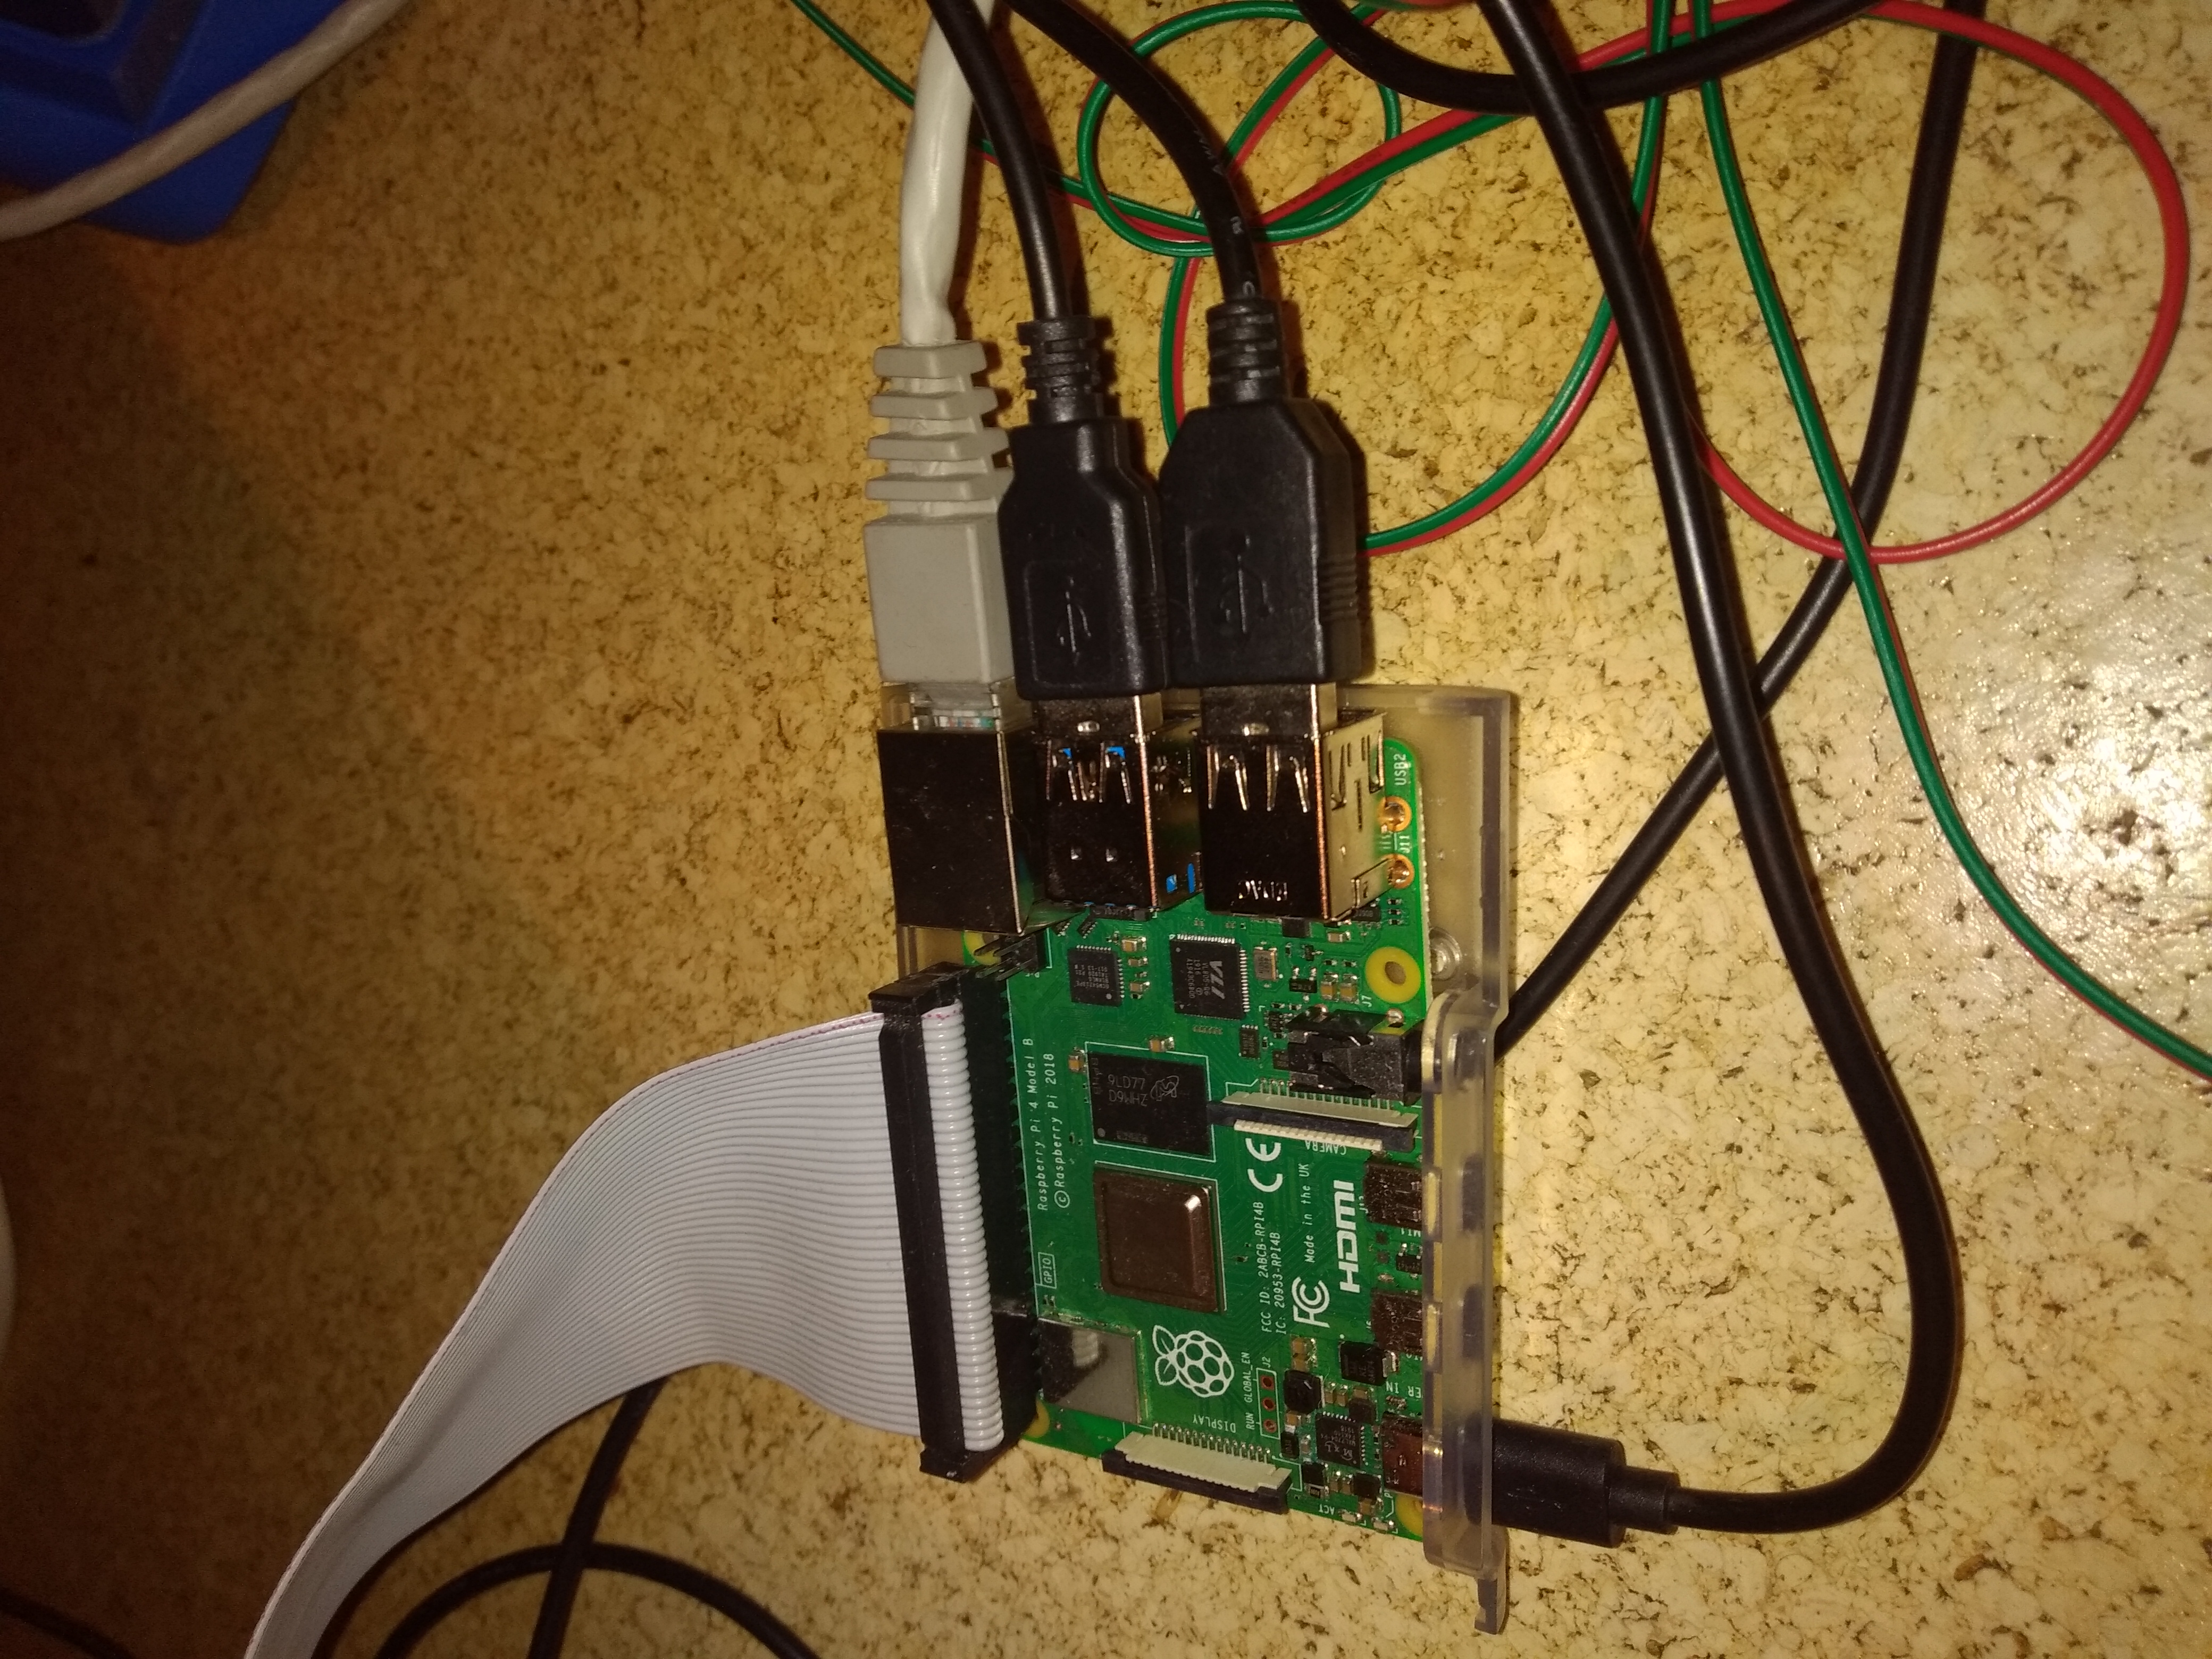
\includegraphics[scale=0.05, angle=180]{raspi}


\subsection{Gartencenter Classic: Universaldünger, leicht säuerlich.}
Dieses Unterkapitel mag Sie etwas überraschen, doch es sei angemerkt, dass mir dieses Thema lange ein Laster war. Die Frage, \textit{wie} und mit welcher Nährstofflösung\footnote{eng. \textit{Nutrientsolution} oder einfach \textit{Solution}} ich meine Pflänzchen füttere, hat mich lange geplagt. Eine einfache Antwort darauf lässt sich im Internet \textit{nicht} finden. Auch \textit{Jeb} hat darauf keine wirklich einfache Antwort, denn er misst die Menge an Kaliumsubstraten mit einer Küchenwage und schmeisst sie dann in den Wasseareimer. Da ich ein Laie in Sachen Substratmixtur bin, brauche ich also eine simplere Lösung, welche mir das Internet nicht gab. Bei einem meiner Besuche in Meiers Gartencenter in Dürnten stiess ich auf \textit{the man himself}, \textbf{Meier}. \\ Er stand hinter dem Kundenberatungsthresen und als ich endlich dran war, ging es keine halbe Minute und er wusste \textit{welche} Solution ich \textit{wo} zu suchen hatte. Gesagt, getan, gefunden, in den Händen hielt ich eine grüne 1L Flasche mit Wunderzeugs. Sie enthält, soweit mich meine Sinne und Kenntnisse nicht trügen, um weitaus mehr Nährstoffe, als alle anderen Dünger aus unserem Gartenschuppen. Das Zeug, mit Leitungswasser vermischt, soll angeblich auch direkt den perfekten pH-Werte haben, 5.5, also leicht auf der sauren Seite. Zu so etwas sage ich nicht Nein. 

\subsection{Löcher im Boden}
Die Pflanzen finden Halt in sogenanannten Steinwolleblöckchen, diese widerum stehen in kleinen Netzbechern/Netcups und \textit{diese} hängen in einem Brett mit Löchern, sodass die Würzelchen im Nährnebel hängen. Das Brett ist aus beschichtetem Holz. Ich habe es zusammen mit dem Zementeimer im Baumarkt gefunden. Zum Leid jeder Nase stank diese Brett so wahnsinnig bestialisch nach einer chemischen Beschichtung, dass ich mehr als einmal keinen Appetit verspürte, nachdem ich die Growbox aufmachte, in der ich alles Material verstaute. Es stank, aber nicht unhygienisch wie gewisse andere Sachen, aber es stank! \\Eines Tages wusste ich, dass ich Löcher in das Brett machen musste. Logisch, das ist ja der Sinn des Brettes. Also ab in den Keller und - Hmm, wie macht ohne es je einmal gemacht zu haben 8cm breite Löcher in chemisch verstärktes Holz? Die Werkstatt offerierte mir einen Bohrer und ein Löcherbohrset, eines mit einer dieser Scheiben, an der man verschiedene, kreisrunde Sägeblätter einstecken kann. Das Problem dabei waren jedoch die vorhandenen Durchmesser, 6cm war das grösstmöglich vorhandene. Mir fehlten also 2cm. \\
Haben sie schon einmal von einer \textit{Oberfräse} gehört? Mein Vater hat so ein Ding und ich habe es gefunden. Dieses Stück Maschine funktioniert im Prinzip wie ein normaler Bohrer, aber seitwärts - mit 12'000 Umdrehungen pro Minute. Anstatt nach unten zu bohren, ist der Fräsenkopf an der Seite mit Klingen bewaffnet, welche sich sterbenshungrig ins Holz fressen. So fest, dass man das ganze Gerät leicht verlieren kann. Denn wenn sich die Fräse erst mal festgebissen hat, gibt es kein entkommen. Die ganze Monstrosität, welche man an zwei (!) massiven Haltern hält, rennt praktisch durchs Holz und es stäubt, oh wie es stäubt. Für die Atemmaske war ich dankbar. Diese Oberfräse ist ein Erlebnis. Das sieht man auch an der tiefen Kerbe in einem der Löcher, der Netzbecher fällt dort fast raus. Den Oberfräsenabend werde ich nicht so schnell vergessen, ich bin noch nie mit so viel Sägestaub aus dem Keller gekommen, meine Augen enthielten mehr Sägemehl als Tränenflüssigkeit.
\newpage










\section{Arbeitsprozess}
Wie genau bin ich wann vorgegangen? Auf diese Frage gibt es viele Antworten, hier sind die wichtigsten. Ich unterteile den Arbeitsprozess in Kategorien, welche widerum Beispiele enthalten.

\subsection{Recherche}
Am Anfang jeder Maturarbeit steht die Recherche. Ich habe, durch YouTube inspiriert, vor allem im Web recherchiert. Mein Wissen, sei es Bewässerung, Optimaltemperatur, Nährstoffe, Belichtungsmethoden, Bewässerungssysteme oder einfach Pflanzen selbst, kam zu einem \textit{sehr} grossen Anteil von Cannabis-Blogs, -shops und -foren. Jeder, der meinen Suchverlauf inspiziert, wird direkt glauben, dass ich vor habe, ganz gross ins THC-Business einzusteigen. Ich kann nicht verleugnen, dass das \textit{Konstrukt} cannabis-bezüglich durchaus Potenzial hätte, aber ich segle lieber \textbf{satt als high}. Deshalb optimiere ich es bewusst \textit{nicht} für sensible Marihuana-Pflänzchen. Es sei auch angemerkt, dass diese Praxis eine Wissenschaft für sich ist, welcher ich mich nicht widmen will. \\ Recherche fand konstant statt, wenn auch nicht immer aufgrund der gleichen Motivation: Am Anfang wollte ich wissen, wie ich das \textit{Konstrukt} überhaupt baue, die Bauteile standen also im Zentrum. Dann hatte es mich mit der Physiologie der Pflanzen an sich gepackt und am Ende verbrachte ich 80\% meiner Web-Zeit auf \textit{stackoverflow.com}, wem diese Webseite ein Name ist, schmunzelt jetzt womöglich - Wem nicht, hier ist die Erklärung: Wenn ein Programmierer auf eine Problem stösst, gibt es eine Website, die in der darauffolgenden Google-Suche \textit{praktisch immer} zuoberst erscheint, es ist \textit{stackoverflow.com}. Die Seite hat über die Jahre anscheinend so ihren Ruf gemacht.¨
Hin und wieder musste ich auch am Ende nicht-programmiertechnische Sachen googeln, aber das war nur etwa ein fünftel, wenn nicht \textit{noch} weniger. Recherche, so trist es auch klingen mag, ist im Bezug auf Debugging z.B. anstrengend und nur das Mittel zum Zweck. Es hilft, den aktuellen Fehler zu finden, aber ehrlich gesagt ist das auch schon alles. Zum Schluss fand ich die Zeit einfach nicht mehr, mich über Pflanzen zu informieren und alles aufzuschreiben. Ich habe anfangs noch alles auf Google-Docs zusammengetragen, habe die Datei \textit{MA-Knowledge} genannt, was für schöne Erinnerungen. Tja - nur mit einem Browser baue ich kein Bewässerungssystem. Dafür brauche ich Kabel, Steckdosen, Relays und einen Lötkolben - und um den geht es jetzt.

\subsection{Löten, testen, löten}
Löten ist, wenn man mit einem heissen Metalkolben Lötzinn, das ist ein Zinndraht mit Flussmittel in der Mitte, zwischen zwei Kontaktstellen verteilt, sodass anschliessend Strom durchfliessen kann. Ich habe zwei eigene Schaltungen gebaut, den PWM- und den Relay-Controller. Beide besitzen als Grundbaustein eine Platine\footnote{Ein 3mm dünnes Plastikbrett mit vielen Löchern}, auf welche ich die Stromleitungen drauflötete. Das an sich ist super cool; Sich selbst einen Schaltplan zu zeichnen und diesen dann in die Realität umzusetzen macht einfach Spass. Mein Vater ist ehemaliger Elektroniker und ich habe mich wie ein Lehrling gefühlt, als er wie ein Prüfer mit dem Finger versucht hat, meine Lötstellen zu durchtrennen, wenn sie hielten war er zufrieden, wenn sie nachgaben und aufsprangen, bedeutete das, dass sie auch keinen Strom durchlassen würden - oder nur begrenzt. Es war eine harte aber effiziente Art, meine Kreationen zu testen. Er vertritt generell die Arbeitsmoral, etwas \textit{einmal, dann aber richtig} zu machen. Und das hat er mir beigebracht. Es gibt keine patzige Lötstelle in keinem Controller, jedes Tröpfchen Zinn sitzt. Der Prozess bestand meistens darin, dass ich im Keller sass, lötete, testete, wenn's gut kam den Fehler selbst fand, nochmal neu lötete und es ihm dann zeigte. Oft musste er mir aber helfen. Ich muss zugeben, die Souveränität und die Art, in welcher ein erfahrener Elektroniker an eine nicht sauber funktionierende Schaltung heran geht, ist beeindruckend. \textit{Ist die Masse überall gleich?} \textit{Ist die Diode verkehrt drin?} \textit{Schau mal diese Lötstelle hier.} Das sind mir indes vertraute Sätze. Wenn ich dann schliesslich mit einer funktionierenden Schaltung hochschritt um sie ihm zu zeigen, war das Gefühl ein besonders schönes. Das Lob eines stolzen Vaters. Ich kann mich wirklich glücklich schätzen, einen Pro im Haus zu haben.\\
Was auch recht half, war die ungeheuer grosse Sammlung an Elektroteilen, welche er noch aus alten Tagen hat. Er hat alle Kisten sortiert, ich konnte ihn einfach fragen, wo die Transistoren sind und er zeigte mir den richtigen. Von Transistoren habe ich vor diesem Projekt zwar schon gewusst, allerdings blieb mir ihre Bedeutung verborgen. Das änderte sich eines Tages, recht am Anfang, als er mir praktisch den ganzen Keller erklärte, angefangen von Dioden, über Transistoren, bis hin zu Spulen. Nicht dass ich jetzt noch besonders viel Details weiss, das muss ich ehrlich gestehen, doch es ist superspannend und recht nützlich zu wissen. Ich weiss jetzt zum Beispiel, wie der Transport via Hochspannungsleitungen funktioniert, respektive \textit{warum} es Hochspannung ist - weniger Energieverluste, so einfach ist das.\\
Ich habe noch etwas anderes gelernt, etwas schmerzhaftes. Aber ganz von vorn. Ich sass eines Nachmittags im Keller, lötete und testete den PWM-Controller und brauchte eine Stromversorgung für die 12V-Lüfter, also brauchte ich ein Netzteil. Netzteile sind oft schwer, was bedeutet, dass es welche sind, welche mit Spulen funktionieren. Ich hatte ein solches rumliegen sehen und prüfte die Ausgangspannung, 12V, passte also. Einmal eingesteckt wollte ich es anschalten, es hatte einen Schalter dran, welcher jedoch nicht \textit{im} Gehäuse, sondern ausserhalb war. Das Netzteil hatte nämlich kein Gehäuse, es war einfach ein Paket Spulen, auf jeder Seite ein Kabel, eins mit 230V und das andere mit 12V und dazu kam der Schalter. Nun ist es so, dass sich der Schalter auf der 230V-Seite befand, also da, wo es richtig weh tut - und das tat es. Der Schalter ist nicht ganz abisoliert worden und beide 230V-Pins waren offen, ich wollte den Schalter mit einer Hand anmachen, musste ihn also mit der gesamten Hand ergreifen, damit ich draufdrücken konnte und ich berührte dadurch direkt die beiden Pins. Es war nicht lebensgefährlich, der Strom floss nur durch meinen Finder, aber es zuckte trotzdem recht schnell. Ich bin noch nie so schnell aufgestanden, wie ein Blitz. Den Adrenalinflash den ich empfand können sich nur andere 230V-Opfer vorstellen; \textit{Huii, das zuckt!} Danach lacht man hysterisch und ist ganz aufgeputscht. Ich muss jetzt noch lachen, einfach irre dieses \textit{Zuck}. Ich habe danach auch verstanden, warum Netzteile in unserem Haushalt \textit{immer} in ein Gehäuse gebaut werden, bevor man sie anschaltet.

%funzt noch nicht richtig

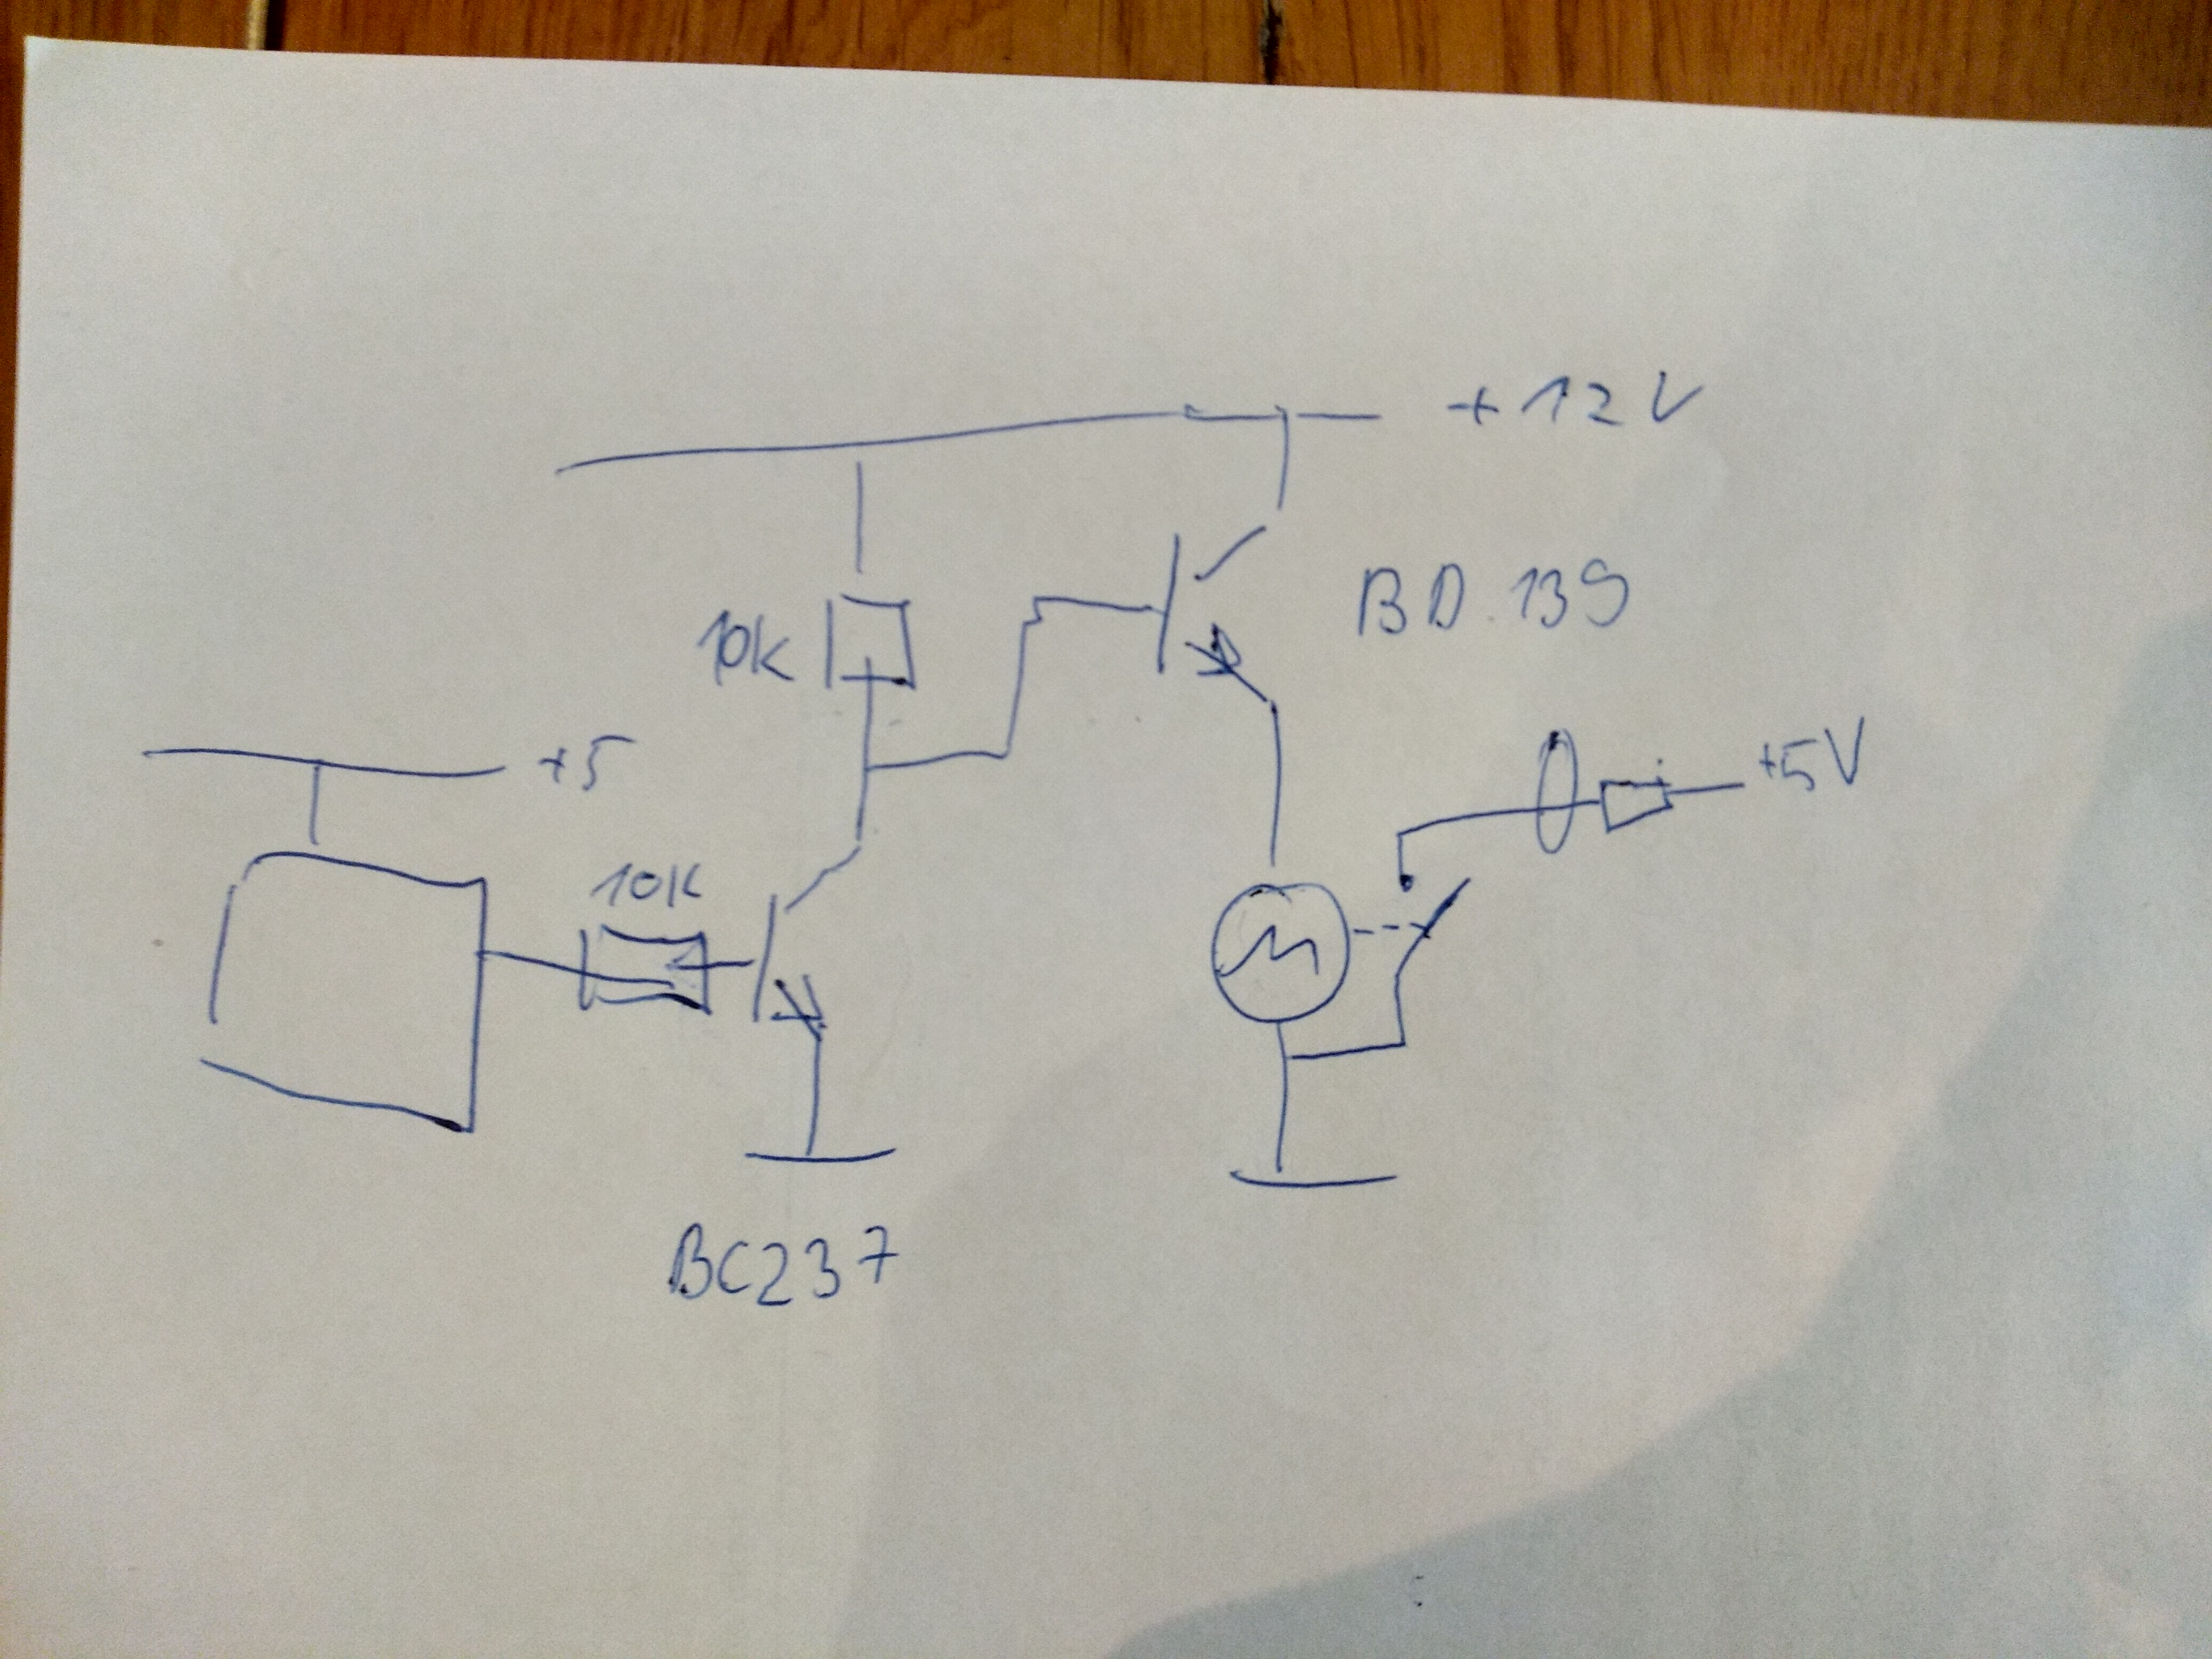
\includegraphics[width=\textwidth, angle=0]{schaltplan}


\subsubsection{Die Hassliebe zu PWM}
Um nun etwas konkreter zu werden, was ich im Keller genau so trieb, werde ich Ihnen nun kurz den Frust beschreiben, welchen meine PWM-Odyssey in mir auslöste. Die Situation ist simpel: Man sitzt im Halbdunkel des Kellers, vor sich der Laptop, der ganze Tisch voller Drähte, Kabel und winzigen Elektroteilchen. Es ist \textit{voll}, eine richtige Unordnung. Das ist normal. Ich teste die Funktionalität der neuen PWM-Schaltung und es geht nicht. Ich sende also genau die Bytes über die serielle Schnittstelle zum Arduino, welche er in PWM-Signale für einen bestimmten Lüfter umwandeln soll. Aber es kommt nicht das von mir erwünschte Ergebnis heraus. Die Frustration ergibt sich nicht aus dem simplen \textit{Nicht-Funktionieren}, sondern aus dem \textit{Wo-ist-der-Fehler?}-Problem. Denn mit einer seriellen Schnittstelle, die sind heikel, glauben Sie mir, einem Arduino, der ist auch heikel, und vier Transistoren hat man reichlich potenzielle Fehlerquellen. Das serielle Signal, also wenige Bytes müssen vom Arduino registriert, gelesen, geparsed\footnote{Mehrere Werte voneinander unterscheiden}, ins richtige Format konvertiert und dann an die PWM-Funktion weitergegeben werden. Diese an sich ist recht schlicht, doch dann erst beginnt der stromtechnische Teil, also die Verteilung der vier PWM-Signale auf die Transistoren, welche den Hauptstrom für die Ventilatoren regeln. Wenn eine Lötstelle nicht richtig verbindet, ist die ganze Leitung unterbrochen, das heisst, dass ich neu löten muss. Und wenn ein ganzer Transistor aufgrund einer zu hoch angesetzten Spannung durchbrennt\footnote{Ich persöhnlich nenne es \textit{frittieren}}, darf man alle drei Pins des Transistors ablöten und einen neuen dranlöten. Puh, das sind eine Menge potenzieller Fehler. Aber ich habe es geschafft, der PWM-Controller tut genau das, was ich ihm jetzt sage. Das ist äusserst erfüllend, auch wenn ich jedesmal noch ein Bisschen Angst habe, auf ein unidentifizierbares Problem zu stossen. Eine technisch genauere Beschreibung dieser Schaltung finden Sie im nächsten Kapitel.

\subsubsection{Relays als nette Abwechslung}
Im Vergleich zum PWM-Karussell war der Relay-Controller um einiges einfacher, wenn man die Software ignoriert... Die Relays, für alle non-Techies\footnote{Wenn Sie diesen Begriff nicht verstehen, sind Sie einer.}, sind wie Lichtschalter, sie lassen entweder Strom durch oder nicht, je nachdem, ob man an einem dritten Pin eine Spannung anlegt oder nicht - hier 5V. Der Lötaufwand war hier um einiges kleiner. Denn ich verwende, weil ich mit 230V arbeite, dickere Kabel, also normale Haushaltskabel. Genau die, welche in ganz neuen, noch lampenlosen Häusern aus der Decke hängen. Sie sind um einiges steifer als meine bisherigen \textit{5V-Drähtchen}. Für den Arduino brauchte ich eine eigene Stromversorgung, welche nicht 230V sondern 5V entspricht. Eigens dafür bestückte ich die Platine mit einem kleinen Netzteil, es ist wirklich niedlich. So richtige Schwieriegkeiten gab es bezüglich der Löt- und Elektronikpraxis beim Relay keine. Was für eine nette Abwechslung.

\subsection{Oszilloskopisches Wunder}
\textit{Das}, lieber Leser, ist ein eigens von mir benanntes Gefühl, welches man empfindet, wenn man das erste Mal einen Fehler findet, indem man sich hinsetzt und versucht, die Stromsignale \textit{selbst} zu verstehen. Wenn man Bedarf für ein solches Gerät hat, weiss man, dass man ganz unten angekommen ist, bezüglich den elektronischen Sphären - Mental ist man nämlich ganz oben. Ein \textit{Oszi} ist ein Gerät mit einem Bildschirm und sogenannten \textit{Klemmen}\footnote{alias Fühler, eng. \textit{Probes}}, welche man an bestimmten Punkten einer Schaltung ansetzt, um anschliessend den Verlauf der Spannung beobachten zu können. Es ist ein Wundergerät, welches jedem richtigen Elektroniker das Herz schneller schlägen lässt. Das beste ist wohl, dass ich jetzt weiss, wie man es bedient. Es hat mir womöglich den Rest meiner Seele gerettet, nachdem ich einen grossen Teil schon verloren hatte und mein Vater mir sagte, wo diese Wundermaschine versteckt ist. Ich benutzte das Oszi für die Veranschaulichung der PWM-Signale. Das funktioniert sehr gut, denn die Verhältnisse lassen sich direkt ablesen. So wusste ich immer, wie stark das PWM-Signal an einem Punkt ist. Bei der Fehlerfindung in einem Labyrinth wie meinem PWM-Controller schätze ich das Oszi besonders. Es wirkt wie eine Leiter, mit welcher man auf Mauern klettert und über die Gänge in Richtung Ausgang balanciert. Das Oszilloskop ist eine Form des \textit{Debuggings}, einer Praxis, welche einen grossen Teil meiner Arbeit ausmacht.

\subsection{Code}
Der Softwareteil des \textit{Konstrukts} ist nicht zu unterschätzen. Ich habe 95\% der Programmierung mit C++ und Python erledigt.

\subsubsection{C++/Arduino}
Der Titel mag etwas verwirren, denn die High-Level-Programmiersprache für alle Arduinos ist eine leichte Abänderung der Sprache C++, welche wiederrum eine objektorientierte Weiterentwicklung des Low-Level-Klassikers \textit{C} ist. Mit dieser Sprache habe ich die \textit{Backends} programmiert, namentlich die Arduinos. Ich verwende zwei, einen für jeden Controller. Beide müssen Signale entgegennehmen und dementsprechend handeln. Am Anfang der Arbeit, ab dem Moment, in dem ich den ersten Arduino herausnahm, lag meine Hauptbeschäftigung fast nur darin, herauszufinden, was ich alles erreichen kann \textit{und wieviel meiner Seele ich dafür opfern muss}. Spass beiseite, ich glaube Sie verstehen langsam, dass mir die Komplexität von Backend-Problemen leicht zuwider ist. Ich erläutere das mal: \textit{C} und das davon abstammende \textit{C++}, respektive \textit{Arduino} sind sehr \textit{lowlevel}, d.h. sie arbeiten nah am Prozessor, für mich als Programmierer bedeutet das, dass ich mich um mehr Probleme sorgen muss, als ich es mir von Sprachen wie Python gewohnt mit. Ein kleines Beispiel habe ich hier. Während bei Python die Deklarierung einer Variable nicht mehr nötig ist,
\begin{verbatim}
number = 5
\end{verbatim}
muss man bei C++ höllisch aufpassen, nichts falsch zu machen, sei es die Deklaration mit \verb&int& oder das \verb&;& am Ende jeder Zeile.
\begin{verbatim}
int number = 5;
\end{verbatim}
Das ist nur eine vieler kleiner Syntaxfinessen, welche einem C++ abverlangt, für mich aus der Python-Ecke ist das kompliziert. Nichtsdestotrotz ist die MA nicht das erste Mal, bei dem ich C++ programmiere, ich kannte auch Arduinos schon davor und habe mit ihnen herumgespielt, z.B. um LED-Streifen anzusteuern. Komplett verloren war ich also nicht. Zudem kommt noch, dass mein Vater jahrelange Erfahrung mit \textit{C} hat. \\Den C++-Code für Arduinos schreibt man in der Arduino-IDE. Diese hat den Vorteil, dass man den Binärcode direkt via USB auf den Arduino hochladen kann. Der Workflow an sich ist somit sehr schnell, was ich schätze. Das grösste Stück Code, das ich schrieb, waren die sogenannten \textit{Relay-Timer}, sie steuern jedes Relay zeitlich unabhängig voneinander. Der Kniff bei der Sache: Wenn man das Problem mithilfe von C++ löst, sind dynamische Änderungen der Grundwerte schwer zu erreichen. Ein Beispiel: Angenommen ein Relay ist für 20s an, lässt also Strom durch, und für 20s aus, lässt keinen Strom durch, und ich verspüre das Verlangen, die Auszeit auf 10s zu ändern; Dann muss die Software, welche den Relays mitteilt, wann sie zu schalten haben, das mitbekommen und seine Konfiguration ändern. Mit C++ ein Protokoll zu erstellen, womit man über die serielle Schnittstelle Kommandos absetzt, in diesem Beispiel eine neue Konfiguration für ein bestimmtes Relay, ist durchaus machbar. Allderdings, und das tut mir in der Seele leid, denn ich verbrachte noch so einige Stunden vor der Arduino-IDE, lässt sich ein so komplexes Problem auf Python einfach besser angehen. Nicht nur sind die Debugging-Möglichkeiten, also das Fehlerfinden, grösser, sondern ich bin schlicht einfach ein besserer Python- als C++-Coder. Was ich also tat, war, das komplette Relay-Timer-Script auf Python zu übersetzen.\\

\subsubsection{Python}
Nicht, dass das Relay-Timer-Script lange gehalten hätte, ich hab's zwei Tage nach der Übersetzung von C++ wieder verworfen und ein komplett neues Konzept zu realisieren versucht. Zu solch code-lastigen Beispielen wie dem Relay-Timer und dem vorher erwähnten PWM-Controller erfahren sie mehr im nächsten Kapitel \textit{Technische Hintergründe}.\\Python ist sehr mächtig und kann vergleichbar schnell von Einsteigern erlernt werden. Gerade in Felderm wie \textit{künstlicher Intelligenz} und\textit{ Big Data} wurde Python in den letzten Jahren immer stärker. Mittlerweile lässt sich fast alles damit machen. Eine Opensource-Bewegung namens \textit{pySerial} hat es sich zum Ziel gemacht, auch noch in den Microprozessor-Sektor vorzudringen, was für mich bedeutet, dass pySerial vielleicht sogar eine ernste Alternative zu C++ dargestellt hätte. Effektiv weiss ich das nicht, denn ich kam mit C++ genug gut klar, als das ich mich hätte umgewöhnen wollen. Python hat also einen grossen Teil der Anforderungen meines Vorhabens erfüllt. Der Workflow ist etwas anders und das Debugging ist einfacher, vorallem mit IDEs wie \textit{PyCharm}. Das ist eine unglaublich umfangreiche Python-IDE von Jetbrains und für meine Vorhaben noch fast zu gross. Das bedeutet, dass ich den letzten grossen Teil Python nicht mit PyCharm sondern mit Sublime bestritt. Sublime ist ein guter Mittelweg, er hat einen eingebauten Compiler, was bedeutet, dass der Code direkt in der IDE ausgeführt werden kann, und ausserdem sind die Editorfunktionen genau nach meinem Geschmack. Jeder Coder entwickelt nach einiger Zeit seine Präferenzen und \textit{mein Gott}, das Sublime-Team hat da ein paar feine Sachen eingebaut! Die intensiven letzten Tage vor der Abgabe habe ich mit Sublime verbracht - Unter Zeitstress muss eine IDE \textit{alles} raushauen können, vor allem \textit{Refactoring}: Wenn man dann einfach mal schnell den Namen einer bestimmten Variabel oder Funktion im \textit{gesamten} Projekt flux ändern kann, dann, lieber Leser, \textit{ist das Premium.}
\\ \\ 
Eine rechte Lobeshymne an Sublime, Sie merken es schon. Was aber \textit{genau} habe ich mit Sublime genau gecodet? Einen Webserver. Schonmal von \textit{Flask} gehört? Das ist eine ganz feine Kreation: Ein Pythonmodul, mit dem man, wie erwartet, einen kompletten Webserver aufsetzen kann. Das trifft sich in meiner Situation recht gut. Ich muss wohl etwas ausholen, denn Sie wundern sich womöglich, warum genau mein Projekt bedarf einer Website hat. \textit{Will er etwa schon sein Smart-Growbox-Business eröffnen?} Nein, das habe ich nocht nicht vor, dafür brauchts noch etwas Entwicklung. Ich könnte die Belüftungsregelung von einer KI übernehmen lassen... \\
Eine Website brauche ich ganz einfach, um einen direkteren Einfluss in die ganze Regelungstechnik zu haben. Beispiele dafür sind die Relays oder manuelle Steuerung des Lüftungsystem. Mit einer Website kann ich von überall der Welt - auch von Korsika aus - auf die Zentralsteuerung meiner Pflanzenlebenserhaltung Einfluss ausüben. \textit{Aber Jonas, was ist mit SSH?}\footnote{SSH ermöglicht es mir remote Textbefehle auf einer Maschine abzusetzen} Ja, liebe Bedenkstimme, SSH, wäre auch eine Möglichkeit, aber damit lassen sich keine Graphen darstellen und ein anständiges, grafisches Benutzerinterface ist einfach was feines. Ausserdem setzt \textit{Flask} auch nur auf Python auf! Eine Website ist einfach cooler und die eben erwähnte Funktion von einer Graphendarstellung \textit{wäre} auch golden. Ich muss Sie jedoch enttäuschen, bis jetzt haben es die Graphen noch nicht auf die Webseite geschafft. Der alleinige Fakt, dass ich mit Python einfach eine Webseite aus dem Boden stampfe ist schon ansehnlich, vorallem weil das ich das vorher noch nie gemacht habe. Und \textit{nur} Python ist es dann eben doch nicht; Das Frontend, also das, was der Browser darstellt, ist ganz traditionell in HTML und CSS geschrieben - und es ist lange her, seit ich das letzte mal Webseiten designed habe. Es wird ja auch immer seltener, dass sich eine Person hinsetzt und echte HTML-Tags in ein Dokument \textit{töckelt}, wenn man die ungeheuere Menge an \textit{Mach-deine-eigene-Webseite}-Angeboten beachtet. \textit{Genau so eine Lösung wäre doch perfekt gewesen, ich hätte mir die Webseite einfach zusammengeklickt}. In erster Linie ja, das Frontend hätte ich so innerhalb eines Tages am laufen gehabt. Den Server allerdings mit den Arduinos zu verbinden, wäre irre schwierig bis unmöglich. Ich brauche meinen eigenen Server. YouTube enthält genug Tutorials, um in zwei Tagen eine solche Web-Instanz ins Leben zu rufen. Ich tat genau das. Zack, hatte ich einen Ordner mit allen nötigen Scripts, um mir selbst eine Seite zu hosten. Das Interface hatte ich auch in \textit{absehbarer} Zeit am laufen. Naja, da fängt eben das Backend des Server an, welches die \textit{wirklich} grossen Aufgaben des \textit{Konstrukts} übernimmt.\\\\
Die Website, wer es noch nicht erraten hat, wird vom Raspi gehostet. Dieses kleine Linux-Gerät kann so einiges, einen Webserver zu hosten ist, wenn man keine ressourcen-lastigen Webapps hostet, ein gutes Beispiel dafür. Jetzt habe ich den Webserver und ein Python-Script, welches die Relays ansteuert. Was fehlt noch? \\
Klar doch, der \textit{Daemon}. Nicht erschrecken, das ist kein echter Dämon, das ist nur ein Hintergrundprozess der, deshalb der Name, \textit{nie stirbt.} Er läuft 24/7. Der Webserver ist auf eine Art auch ein \textit{Daemon}, er läuft auch immer, sonst wäre es eine seltsame Webseite. Eine Website mit Öffnungszeiten, komische Vorstellung... Der Daemon ist das Herz, das Hirn, nennen Sie es wie Sie wollen. Er läuft immer, weiss und steuert alles. Ich habe den natürlich auch in Python geschrieben. Der Webserver und das Relay-Script waren im Vergleich zum Daemon kleine Engel. Das ganze Ding ist so komplex aufgebaut, dass ich einiges meiner Seele opfern musste, bis ich den Dämon bezwang... Im Technik-Kapitel erfahren Sie genauer, wie er funktioniert. Jetzt geht es weiter mit Git - dem nächsten Biest.


\subsection{GitHub, the Beast}
Der Titel soll nicht lügen. Wenn Sie jemals mit Git gearbeitet haben, dann stimmen Sie mir zu, wenn nicht, erkläre ich es kurz. GitHub ist ein Onlinedienst, auf das man seine Code-Projekte hochlädt, um mit einem Team, Opensource-Community oder auch ganz allein daran zu arbeiten. Es erlaubt einem eine fortgeschrittene Kontrolle über verschiedene Versionen des Projekts. Ich habe den kompletten Datenteil des \textit{Konstrukts} mit Git verwaltet, also jedes Stück Code, Bilder, Konzepte und auch alle LaTeX-Dateien, respektive die Buchstaben welche Sie \textit{jetzt} gerade lesen. Es funktioniert wie eine grosse Cloud, einfach besser und mit einer Menge mehr Funktionen. So viele, dass ich einen guten Teil meiner Zeit damit verbrachte, \verb^git^ \textit{zu lernen}. Man achte auf die Kleinschreibung, denn ich rede vom \textit{Program/Protokoll} \verb?git?. Das gesamte Thema \textit{GitHub-Versioncontrol} ist eine Welt für sich. Eine Wissenschaft so wie die Materie der Elektronik, die Pulsweitenmodulation(PWM), die erwähnte Marihuana-Praxis derer, die es ernst damit meinen, dem Coden von Python, C++ oder HTML. Auf die erlernten Fähigkeiten wird im Kapitel \textit{Perspektiven} noch eingegangen. Das es in diesem Kapitel um den Arbeitsprozess und meines Erachtens deshalb auch um den \textit{Workflow} geht, sind hier die wichtigsten \verb?git?-Befehle.
\begin{verbatim}
git clone
\end{verbatim}
\textit{Gecloned} wird ein Repo (eine Code-Sammlung), wenn man es zum ersten Mal runterlädt.
\begin{verbatim}
git commit 
\end{verbatim}
\textit{Committen} macht der Programmierer, nach jeder mehr oder weniger substantiellen Änderung. Das Hochladen erfolgt mit
\begin{verbatim}
git push
\end{verbatim}
Und falls es aus der Cloud gespeicherte Änderungen lokal zu synchronisieren gibt, benutzt man
\begin{verbatim}
git pull
\end{verbatim}
Um zwischen verschiedenen Versionen, auch \textit{Branches/Äste} genannt, umherzuswitchen, benutzt man
\begin{verbatim}
git checkout
\end{verbatim}
Dies sind die wichtigsten Befehle, welche ich während meiner gesamten Developement-Phase verwendet habe. Natürlich ist das nur die Spitze des Eisbergs, Git birgt noch so manche, deshalb nenne ich es auch \textit{the Beast}. Es erleichtert vielen Developern ungemein die Arbeit. Das nächste ist ebenfalls eines davon.

\subsection{Bash}
Nebst all den Programmiersprachen, dem Lötkolben und dem Oszilloskop verdanke ich der \textit{Bash}einen ungemein grossen Teil meiner Effizienz.
\begin{verbatim}
jonas@pop-os:~$
\end{verbatim}
Jedes Mal, wenn ich das Terminal öffne, grüsst mich dieser Prompt, was dann folgt sind meistens Kommandos wie \verb&cd& oder \verb&ls&. Unter Zeitdruck werden sie so schnell in die Tasten genagelt, dass ich fast Mitleid mit meiner Tastatur habe. Auch hier wird mir jeder geneigte \textit{Linux-Pinguin} einfach nur zunicken und kaum merklich schmunzeln. Die oben genannten Commands, für alle welche nicht vom Südpol stammen, sind die Augen und Beine in der Bash, mit \verb&cd& läuft man durchs Dateinsystem und mit \verb&ls& verschafft man sich einen Überblick über alle vorhandenen Dateien in einem bestimmten Ordner. Die Bash hat eine \textit{so} grosse Präsenz in meinem Leben, wie kein anderes Programm, naja YouTube vielleicht: Jeden \verb^git^-Command setzt man über die Bash ab. Man navigiert damit durch den Computer, tötet überflüssige Prozesse (aber ja nicht die Dämonen, versteht sich) oder programmiert mit \verb&vim& oder \verb$nano$ kurz ein kleines Bash-Script. Ich habe genau einmal ein Bash-Script gebaut und zwar, als es mir zu blöd wurde, via GitHub meinen Daemon-Code auf den Raspi zu laden.
\subsubsection{rsync}
\verb^rsync^ ist Dropbox für die Kommandozeile/Bash, einfach cooler: Es kann verschlüsselt und rekursiv Daten von einer Quelle zum Ziel kopieren, alles was schon da ist, wird nicht doppelt kopiert. Es ist äussert flink und einfach zu bedienen, wenn man sich dann mit den \textit{SSH-Keys} richtig anstellt, muss man nichtmal das Passwort des Zielrechners angeben. Das von mir vorher erwähnte Bash-Script hat alle 5 Sekunden meine Änderung, welche ich mit Sublime, Gott hab es seelig, am Dämonen (ich verwende absichtlich das böse Wort) vorgenommen hab, auf den Raspi kopiert. Was habe ich mir damit gespart? Einen kompletten  \verb^git commit -a && git push^ Befehl, zusammen mit dem \textit{Commit-Kommentar}, den \verb&git& jedes Mal von einem verlangt, wenn man die Änderungen committet. Rundherum sind das grob 10s und eine Menge unnötiger Tastenanschläge, denn ein GitHub-Commit für lediglich die Änderung eines Variabelnamens war in meiner Situation einfach ein \textit{Overkill}. Vielleicht sollte ich den Workflow zusammen mit dem Raspi kurz erläutern: Den Dämon habe ich auf meine Laptop mit Sublime und Seelenopferung beschworen. Ich glaube wir kommen humorstechnisch langsam auf eine Welle. Wirklich funktioniert hat der Dämon aber nur auf dem Raspi, denn da sind auch die Sensormodule installiert, mit welchen der Dämon die Lüfterstärke berechnet (mehr technische Details im nächsten Kapitel). Da diese Module auf meinem Laptop keinen Sinn machten, war die Beschwörungsumgebung auf meinem Laptop, die Testumgebung aber auf dem Raspi. \verb^rsync^ war quasi die Geisterbrücke zwischen seiner Höllenschmiede und seiner Herrschaftsdomäne, um es ganz theatralisch auszudrücken. Das mit dem Schmieden ist so eine Sache, denn die Anzahl Bugs und Imperfektionen im Dämonen trieben mich fast in den Wahnsinn. Deshalb musste ich ja erst so oft hin- und herswitchen, \textit{testen, fixen, testen, fixed} - ein höllisches Karussell, versteht sich. Bitte verzeihen Sie mir die, aus gutchristlicher Sicht, viellieicht respektlosen Bemerkungen bezüglich des ganzen Höllen-Tatas, ich bin nicht gläubig, also teufelsfürchtig und möchte keinem auf die Füsse stehen. \verb^rsync^ hat mir das Leben sehr erleichtert.

\subsubsection{Secure Shell - SSH}
Es ist so weit. Eine weitere Lobeshymne findet ihren Anfang. Ich habe das leichte Gefühl, dass dieses ganze Kapitel eine Danksagung ist. SSH bedeutet, wie im Titel schon angemerkt, \textit{Secure Shell} und der Name wird der Software gerecht. Ich bin nicht hier, um Ihnen klar zu machen wie massiv der Einfluss von SSH auf die heutige Internetkultur ist, deshalb fasse ich mich kurz: Es ist wie der Sicherheitsgurt beim Auto. Denken Sie bitte darüber nach und lesen Sie dann weiter. Die Lobeshymne können Sie sich wahrscheinlich auch schon selbst zusammenreimen. Doch fragen Sie sich bestimmt auch, wie und warum ich dieses Protokoll einsetzte. Zuerst den genauen Sachverhalt: SSH benutzt praktisch jeder Sysadmin dieser Welt, um sich auf einem Remotesystem einzuloggen oder darüber Daten zu verschieben. Des Weiteren wird das Protokoll selbst für \textit{Portforwarding- und Tunnelingzwecke} eingesetzt, das muss Ihnen nichts sagen und ich werde es auch nicht erklären, aber googeln Sie es einfach. Das mit dem remote einloggen ist der Grund warum ich es benutze, hat man auf dem Zielsystem, in meinem Fall der Raspi, einen \verb^openssh-server^ am laufen (ja das ist auch ein Daemon :), kann man auf dem lokalen System einfach so tun, als hätte man eine Bash im Remotesystem - Man setzt also verschlüsselt Bash-Befehle auf ein anderes System ab. Simpel. Der Raspi hat zwar eine grafische Oberfläche, das RaspbianOS, doch ich hatte nur einen Monitor, welchen ich schon als Workstation für meinen Laptop verwendete. Deshalb war SSH der einzige Zuga- \textit{Aber Jonas, was ist mit VNC?} Ach ja, die Bedenkstimme. Klar, VNC hätte auch funktioniert. Das ist SSH, einfach grafisch. (Benutzt den SSH-Tunneling-Aspekt, aber psst!) Ich habe es mit VNC versucht, es hat nicht geklappt und ich habe es aufgegeben. Wahrscheinlich wäre es auch sehr stockend gewesen und Lags kann ich in der letzten Developement-Phase nicht gebrauchen, ich verlange Sublime-Standarts und die hätte mir VNC sehr wahrscheinich nicht geliefert. Aber SSH tat es, so wie immer. Durch die textbasierte Oberfläche, müssen keine grafischen Daten durch die SSH-Leitung, also ist alles schneller, wenn man den Raspi dann noch mit einem Ethernet-Kabel betreit, also nicht über WiFi, fliegt man zum Mond. Die konventionelle Benutzung von SSH kannte ich schon von früher - ich bin ein Linuxkind - aber das \textit{Keymanagement} hat während diesem Projekt eine neue Anekdote bekommen. Im vorherigen Unterkapitel \verb/rsync/ habe ich kurz von SSH-Keys geschrieben und ich möchte den unwissenden Leserseelchen genüge tun, indem ich Ihnen die Genialität hinter dem Private- und Publickeyprinzip von SSH  erklären. Sie liegt nämlich in der Einfachheit des Systems. Ich generiere als erstes meine Keys. Es sind zwei, ein privater und ein öffentlicher. Der öffentliche kann ich auf dem Raspi in eine Datei schreiben, womit er alle Daten, welche er mir schickt, verschlüsselt. Die von meinem öffentlichen Key verschlüsselten Daten werden, bei mir angekommen, von meinem privaten Key einfach wieder entschlüsselt. Deshalb sollte man den Privatekey auch nie weitergeben, denn sonst könnten andere Leute \textit{meine} Daten entschlüsseln. Um bei \verb/rsync/ also nicht immer das Passwort des Raspis eingeben zu müssen, hinterlege ich dort meinen Publickey und mache mir um Sicherheitsrisiken keine Sorgen mehr. Der Datentransfer ist verschlüsselt und zwar mit so hohen Verschlüsselungsraten, dass schon bei einem, heute fast überall gebräuchichen \textit{RSA-2048 Algorithmus} keine menschliche Technologie ausreicht, um ihn in absehbarer Zeit zu knacken. Ich behalte es mir vor, diese Aussage auch auf Quantencomputer zu beziehen, aus Unsicherheit ob meine Aussage korrekt wäre.

\subsubsection{Tilix}
\textit{Tilix} ist weder ein Bashprogram, noch ein Protokoll. Es ist vielmehr ein Program für die Bash, ein grafisches Fenster, worin man die Bash benutzt. Das spezielle an \textit{Tilix} ist das \textit{Multiwindow-Feature}, anstatt dem traditionellen \textit{Eine-Bash-Ein-Fenster}(von Tabs mal abgesehen) kann ich hier den ganzen Bildschirm ausfüllend ein Bashfenster neben dem andern haben, alles noch im Tilix-Fenster selbst. Damit habe ich mich in verschiedenen Bashfenstern per SSH auf dem Raspi eingeloggt, um parallel Kommandos abzusetzen und Daten auszulesen, z.B. die Statusmeldungen des Flask-Webservers. Es ist recht gemütlich, alle Terminals (alias Kommandozeilenfenster) auf einem Bildschirm zu haben.

\subsection{Forschung}
Ich habe nicht wirklich geforscht, nicht wissenschaftlich jedenfalls, ich habe lediglich verschiedene Setups aufgebaut um zu sehen, welches am besten funktioniert. Konkret ging es um die Bewässerungszyklen, also um die Frage, wie lange ich den Fogger ausgeschalten lassen kann, bevor ich ihn wieder anstellen muss, damit genug Nährnebel für die Würzelchen da ist. Sie sollen ja nicht austrocknen. Der Nebel, so trocken er auch ist, kondensiert nach einer Weile und die Trockenheit bekommt den Pflänzchen nicht gut.. Ich nenne es Forschung, weil es sich gut anfühlt, behaupten zu können, \textit{dass man jetzt in den Garen forschen geht.} Ich hoffe Sie verstehen meine Kindlichkeit.


\subsection{LaTeX}
Wie man am Layout dieser Arbeit vielleicht schon gemerkt hat, schreibe ich alles mit LaTeX. Beim Rechercheprozess und im Gespräch mit meinem Vater stiess ich zuerst auf den Namen. Der Name ist \textit{catchy}, ich hatte ihn zuvor also schon mal gesehen, mich aber immer gewundert, was es bedeutet. Auf gutes Zureden meines Vaters wagte ich es schlussendlich, mir dieses Wunderwerkzeug genauer anzuschauen und es überzeugte mich. Der Fakt, dass ich mir um das Layout keine Gedanken machen muss und es dennoch gut aussieht, ist mir sehr möchtekommen. Es hat alledings ein paar Tage gedauert, bis ich den Workflow verstand und auch jetzt beim wirklichen Schreibprozess habe ich immer wieder Fragen.§

\subsection{Logging}
ASDFASDFASDFASDF


\section{Technische Hintergründe}
Also gut, es geht los. Ich hoffe Sie sind bereit, eine Menge Technik zu lesen. Hier schildere ich jedes Modul und dessen Funktionsweise. Ich denke, ich erkläre Ihnen am besten zuerst die Arbeitsweise des \textit{Konstrukts}. Zwischendurch lockere ich es mit einem kleinen Seitenfakt auf.
\subsection{Ganz von vorn.}
Das \textit{Konstrukt }stellt für entweder vier oder acht Pflanzen möglichst optimale Wachstumsbedingungen her. Diese Ansprüche habe ich bereits geschildert, nun geht es darum, wie sie garantiert werden.
\subsection{Bitte nicht reinschauen}
Schauen Sie ihren eigenen Netzhäuten zuliebe \textit{nicht} direkt in Growing-LEDs, für Ihre Augen ist es etwa so, als müssten Sie mit der Hand ein Panzergeschoss stoppen. Die LEDs habe zwar keine Laser-Klassifizierung, aber das ändert nichts am Leuchten, das Sie während den anschliessenden 5Minuten auf der Netzhaut spüren, nachdem Sie kurz neugierig waren.\\LEDs sind cool. Sehr Effizient in Sachen Energie, was zur Folge hat, dass weitaus mehr Elektrizität in Licht und nicht in Wärme umgewandelt wird, als bei herkömmlichen Halogenlampen oder dergleichen.. In der Natur gewöhnen sich Pflanzen an das Abwechselnde Hell-Dunkel von Tag und Nacht. Es bewirkt eine stabilisierung des Pflanzenkreislaufs, denn, und das habe ich vorher nicht gewusst, Pflanzen können zu viel Licht bekommen. Es klingt Merkwürdig, aber es macht Sinn: Ein Blatt in all seiner Genialität, ist bei weitem nicht perfekt. Bei zuviel Sonneneinstrahlung geraten gewisse Arten an Teilchen innerhalb des Kreislauf ausser Kontroller und blockieren z.B. die Zufuhr von Kohlendioxid. Genau möchte und kann ich das selbst nicht erklären. Kurz gesagt: Wir müssen diese LEDs einfach mal abschalten können, sonst tue ich den Blättchen das Gleiche wie meinen Netzhäuten an. Die LEDs sind einfach Lampen in einem flachen Gehäuse, an dem ein Kabel angeschlossen ist. Dieses Kabel stecke ich in den Relay-Controller, dessen Relays den Stromfluss auf die jeweilge Steckdose kontrollieren. In den Weed-Foren habe ich von einem Belichtungszyklus von 18h zu 6h gehört, was ungefähr auch meinem Schlafzyklus entspricht. Meine Pflanzen gehen also mit mir ins Bett. Per Webinterface programmiere ich die \textit{ontime} auf 18h * 60min * 60s, was insgesamt 64800 Sekunden sind. Ausgeschaltet sind sie demnach 21600 Sekunden. Vorerst benutze ich die LEDs immer abwechselnd, es muss hier ja nicht noch jemand/etwas die Seele verlieren.. Das Gute an meinem System ist jetzt schlicht der Fakt, dass ich die Belichtungszeit einfach ändern kann. Ich kann sie so einstellen, dass die Lichter aus sind, wenn ich ins Bett gehen möchte. Die Growbox ist zwar recht dicht, doch bei den Reissverschlüssen leuchtet es dennoch etwas durch, von den Lüftungslöchern mal ganz abgesehen. Wirklich heiss werden die LEDs auch nicht. Das Lichtspektrum ist wie schon in der Bauteilliste so eingestellt, dasses genau dem von den Pflanzen benötigten Wellenlängen entspricht. Es gibt eine ganz einfache Methode um herauszufinden, ob die Blätter das Licht absorbieren oder nicht. Wenn sie es \textit{nicht} absorbieren, dann müssen sie es reflektieren. Wenn die Blätter also schwarz erscheinen, weil sie nichts reflektieren und alles absorbieren funktionieren die eingestellten Wellenlängen.


\subsection{Das Ding atmet ja!}
Wir Sauerstoff-Atmer existieren aus dem alleinigen Grund, dass Pflanzen CO$ _{2} $-Ein- und O$ _{2} $-Ausatmer sind. Was sie als O$ _{2} $ \textit{ausatmen} brauchen wir, damit unsere Mitochondrien aus Glucose ATP, einen chemischen Energieträger machen können.
Die Growbox hat ein Leervolumen von 0.612m$ ^{3} $, das ist nicht viel und man sollte auch bedenken, dass da noch ein kompletter Zementeimer drin steht, welcher von einem Brett bedeckt wird, welches die Box glatt in zwei Teile teilt. Von den 170cm Höhe verliere ich also gute 35cm, was mich mit nichtmal einem halben Kubikmeter zurücklässt. Das CO$ _{2} $ ist deswegen schnell aufgebraucht und es wird auch schneller heiss. Wenn das CO$ _{2} $ aufgebraucht ist, betreiben die Pflanzen keine Photosnythese mehr. Diese Situationen gilt es demnach zu vermeiden. Der komplette Luftzyklus ist aufgrund dem sich ausdehenden Verhalten von Luft, aufwärts gerichtet. Unten kommt die kältere, CO$ _{2} $-reiche Luft und oben wird die wärmere, CO$ _{2} $-arme Luft rausgeblasen. In richtig grossen Anlagen wird nicht nur aus CO$ _{2} $-Gründen gelüftet, sondern auch, weil es zu heiss werden kann. Bei mir ist das mit meinen 50W-LEDs aber komplett nicht der Fall. Für die Photosynthese essenzielle Proteine verlieren ihre Tertiärform, die Form die ihnen ihr Funktionieren ermöglicht, ab etwa 35°C. Ich gehe stark davon aus, niemals an diesen Wert zu gelangen. Auch wenn mein Zimmer, der Standort des \textit{Konstrukt} im Sommer recht heiss werden kann, reden wir von maximal 30°C. Ich behaupte nicht, dass es unmöglich ist, die Schmerzgrenze von 35°C in meinem Zimmer zu erreichen, aber durch die eingebaute Thermostatenfunktion des Dämons werden wir ein \textit{Meltdown} der kleinen, guten Proteinchen meiner Pflanzen hoffentlich nie erleben.

\subsubsection{Die Zauberformel mag es lieber trocken}
Während der gesamten Konstruktionsphase und einem guten Teil der Schreibphase war ich im Glauben, schon bei niedrigen Temperaturen durch lüften, kühlen zu müssen. Jüngste Erkenntnisse widerlegen diesen Glauben, dennoch möchte ich Sie mit meinen Gedanken im Bezug auf den Relevanzunterschied zwischen Temperatur und relativer Luftfeuchte bekannt machen. Die Signifikanz der Luftfeuchte auf das Wachstum \textit{meiner} Pflanzen in \textit{meiner Konstruktumgebung} hat sich ebenfalls geändert, doch wir sind hier im Kapitel des Arbeitsprozesses, in dem ich Ihnen direkte Einblicke in meine Gedanken ermögliche. Lesen Sie das folgende mit dem Wissen im Hinterkopf, dass sich \textit{auch} die Signifikanz der Temperatur verringert hat.\\\\
Ein komplett anderer Luftaspekt ist die relative Luftfeuchte, ich kürze das mit rel. LF, ab. Ich nehme an (!) dass es Pflanzen beim Stoffwechsel hindert, wenn die Luft zu feucht ist. Hier ein Erklärungsversuch: Innerhalb der Pflanze werden Bausteine und Wasser über den Stängel wie auf einem Fliessband transportiert. Das Wasser an sich ist schon ein essenzieller Faktor in jedem Stoffwechsel. Die ganze Überlegung macht mehr Sinn, wenn man weiss, dass der Sog innerhalb der Pflanze nur dadurch entsteht, weil Wasser an der Unterseite der Blätter kondensiert und so \textit{neues} Wasser \textit{nachgesogen} wird, das hat mit sogennanten Kapillarkräften zu tun, welche es dem Wasser erleichtern, durch sehr dünne Kanäle zu fliessen. Wenn die rel. LF aber zu hoch ist, kondensiert das Wasser an der Blattunterseite nicht mehr, weil es, vereinfacht angeschaut, keinen Platz mehr in der Luft hat, wo sich noch mehr Wassertröpchen aufhalten könnten. Der Kapillarfluss kommt also ins Stocken und die Pflanze wird am Wachstum gehindert. Ich bin mir bei dieser Überlegung nicht sicher, was mich dazu bewegte, die rel. LF einfach aus der Gleichung zu entfernen. Ich mag es simpel. Es ist von einer ganz bestimmten Gleichung die Rede, nämlich der Vorgang, bei dem der Dämon, da ist er wieder, berechnet, wieviel Saft (in Form von PWM) er denn Lüftern geben muss. Schlussendlich, auch wenn ich die nötige Technologie besass und zur Hand hatte, habe ich mich einfach dazu entschieden, diesen kompletten Aspekt zu streichen. Vorallem auch deswegen, weil ich nach einer Beispielsberechnung gemerkt habe, dass die LF einen \textit{viel} zu geringen Einfluss auf das PWM-Signal hat. Es ist wohl am besten, wenn ich das kurz erläutere und da wir hier im technischen Teil sind, werden Sie sich alle Mühe machen, es auch zu verstehen. Vorerst möchte ich anmerken, dass alle von mir genannten Werte meine eigenen Annahmen sind und womöglich komplett daneben sind, ich habe noch nie ein Belüftungssystem gebaut. Los geht's\\Die Lüfter laufen konstant auf 40\% PWM, um den Pflanzen genügend CO$ _{2} $-Zirkulation zu geben. Alles was daraufgerechnet werden, also die restlichen 60\% hängen von der Temperatur ab. Mit der Temperatur mache ich es so, dass ich einen Optimalwert halten möchte, ich ging in meinen Berrechnungen meistens von etwa 24°C aus, wie gesagt, dieses Milieu ist mir neu. In Relation zu diesen 24°C gehe ich von einer Temperatur aus, ab welcher ich auf voller Stufe lüften möchte, sagen wir 27°C, es bleiben uns also 3°, welche wir auf unsere 60\% verteilen: Einfache Proportionalität, wir gehen also davon aus, \textit{pro jedem Grad über dem Optimalwert 20\% PWM-Saft auf die schon bestehenden 40\% zu addieren}. So einfach habe ich mir das Leben gemacht. Eine ähnliche Überlegung bin ich bei der rel. LF eingegangen, allerdings sind meine Kenntnisse da noch weniger und der effektive Wert, um welchen ich mehr lüften muss, war ca. ein Zehntel dessen der Temperatur-Überlegung. Ich hatte anfangs beide in der Berechnung drin, da aber die Temperatur einen grösseren Impact hat, musste ich auch diese Einflussdifferenz berücksichtigen, was den Dämonen nurnoch verkomplizierte. Und lassen Sie mich Ihnen versichern, dass dieses Dämonenwerk auch ohne Lufteuche-Berücksichtigung schon kompliziert genug ist, jedenfalls für mich.
Ein realistischer Daten-Ablauf sieht folgendermassen aus: Der Dämon läuft in einer Endlosschlaufe und fragt den an den Raspi angeschlossenen DHT22-Temperatur \& rel. LF-Sensor nach der Temperatur. Diese zusammen mit den Werten der Standart-PWM-Frequenz, dem Wunschwert und dem angenommenen Full-PWM-Wert (Ab da wo die Lüfter voll durchschalten) verrechnet er zum sogennanten \textit{Auto-PWM-Wert}. Die automatische Berechnung dieses Werts lässt sich per Web-Interface deaktivieren. Dieser Auto-PWM-Wert wird anschliessend vom Dämonen an den PWM-Controller weitergegeben, über eine serielle Schnittstelle, alias USB-Kabel, welche ich beim Start des Dämons iniziiere und dann offen behalte, bis der Dämon stirbt - was natürlich \textit{nie} passieren wird, versteht sich.\\
Wer aufmerksam gelesen hat, bemerkt vielleicht, dass ich bisher nur von zwei Lüftern schrieb, jedoch erwähnte ich in der Bauteilliste \textit{vier}, was also machen die zwei anderen Lüfter? Von einem kann ich es Ihnen schon verraten, beim anderen müssen Sie sich noch etwas gedulden. Der dritte Lüfter hat eine ganz einfache Aufgabe, er innerhalb der Growbox für Turbulenzen sorgen und die Pflanzen direkt beblasen. Ich habe diesen Tipp ganz tief aus einem dieser 420-Portalen, anscheindend werden die Pflanzen damit stabiler und gesünder, was an sich Sinn ergibt. Ein Mensch ist auch gesünder wenn er Widerstand leisten muss, zum Beispiel beim Sport treiben. Wenn einem Organismus etwas abverlangt wird, entwickeln sich daraus Reserven, um dieser Situation nicht mehr ausgeliefert zu sein. Um also nicht einfach umgewindet zu werden, baut die Pflanze stabilere Wände.

\subsection{Vom Gravitropismus und der Zukunft}
An dieser Stelle passt es wohl am besten, um Ihnen vom \textit{Gravitropismus} einer Pflanze zu berichten. Dieses Wort beschreibt die Reaktion von Pflanzen auf unterschiedliche Richtungen in denen die Gravitation auf sie einwirkt. Haben Sie schonmal einen schrägen, oder sogar ganz umgewehten Baum gesehen, bei dem die Äste dennoch gen Himmel wachsen? Ich mache es Ihnen noch einfacher: Wenn immer eine junger Baum an einer sehr steilen Stelle wächst und sich, einfach aus Platzgründen, senkrecht zum Untergrund emporhebt, was aber \textit{nicht} senkrecht zum Horizont ist, dauert es nicht lange und er wächst wieder gerade in den Himmel. Dieses Ausrichten trägt den Namen \textit{Gravitropismus} und es funktioniert, indem die Pflanze an der Stelle mehr Zellen produziert, von welcher sie weg möcht, was für uns als \textit{unten} bekannt ist. \textit{Unten} an einer Pflanzen bildet sich mehr Masse, was den gesamten Stamm/Stiel/Ast in die andere Richtung drückt. An der Aussenseite einer Kurve hat es mehr Material als an der Innenseite, deshalb ist die Innenseite einer Kurve auch der kürzeste Weg. Stellen wir uns kurz die Frage, wer von diesem \textit{Gravitropismus} Gebrauch machen könnte. Es sind neue, vertikale Farmen, mit dem Ziel, möglichst viel Nahrung auf möglichst kleinem Raum zu produzieren. Diese neuen Anlagen bringen ihre Pflanzen in unterschiedliche Ausrichtungen, wodurch sich die Einwirkung der Gravitation ändert und somit der Gravitropismus. Im Ende versuchen die Pflanzen, nebst dem normalen Wachstum auch noch nach oben zu wachsen, was zu mehr Pflanzensubstanz führt. Genial, nicht? Gerade auf einem Planeten wie der Erde, mit ihrer immer grösser werdenden \textit{Wie ernähren wir alle 11 Milliarden Erdlinge im Jahre 2100?}-Frage, sind Erkenntnisse wie diese sehr erwünscht.






\subsection{Wurzelfütterung}
\subsubsection{Nährnebelpegel}
Wenn die Wurzeln noch jung, also noch \textit{kurz} sind, muss ja rein theorethis der Pegel an Nährnebel höher sein, damit er sie erreicht. Aber das hätte zur Folge, dass ich die Relays, auch wenn es super einfach ist, umprogrammieren muss. Hier kommt der vierte Lüfter ins Spiel. Eher gesagt ist es en Lüfterchen, auf dem Querschnitt unten ist er ebenfalls zu finden und dort erkennt man auch schon seine Funktion. Er schafft wie der dritte Lüfter Turbulenzen, allerdings im Nährnebel, um ihn damit weiter nach oben steigen zu lassen. Ich habe dieses Phänomen schon das erste Mal, als ich den Fogger eingestellt habe, beobachtet. Wenn man ganz heiss darauf ist, ein neues Spielzeug auszuprobieren, wartet man nicht lange. Meine Mutter wartete darauf, dass ich zum Essen komme, doch der frisch mit der Post angekommene Fogger war da. Einmal eingesteckt und in eine Wasserschüssel gesetzt schaltete ich ihn ein. Es sieht wie ein kleiner Vulkan aus, wenn das Wasser so hoch spritzt. Die ganz kleinen Tröpfchen, die mit einem Zweihundertstel Millimeter Durchmesser machen sich als Nebel bemerkbar und der Rest spritzt als ganz herkömmliches Spritzwasser hoch. Nach ein paar Sekunden Laufzeit hat sich eine ordentliche Menge Nebel angesammelt und jeder Mensch, der auch mal ein Kind war, spürt das unbekämpfbare Verlangen a) hineinzufassen und b) hineinzupusten. Gesagt, getan, die ganze Küche sieht leicht milchig aus. Mit künstlichem Nebel herumzuspielen ist irre witzig. Die Erkenntnis aus diesen Spielerein lag ganz einfach darin, dass man den Nebel recht einfach anheben kann, indem man ganz leicht in die Mitte bläst, auf der Darstellung ist das genauso illustriert. Die Bretter, durch welche ich die Netzbecher stecke, in denen die Steinwolleblöckchen sind, in denen widerum die Pflanzen halt finden, haben entweder fünf oder neun Löcher. 
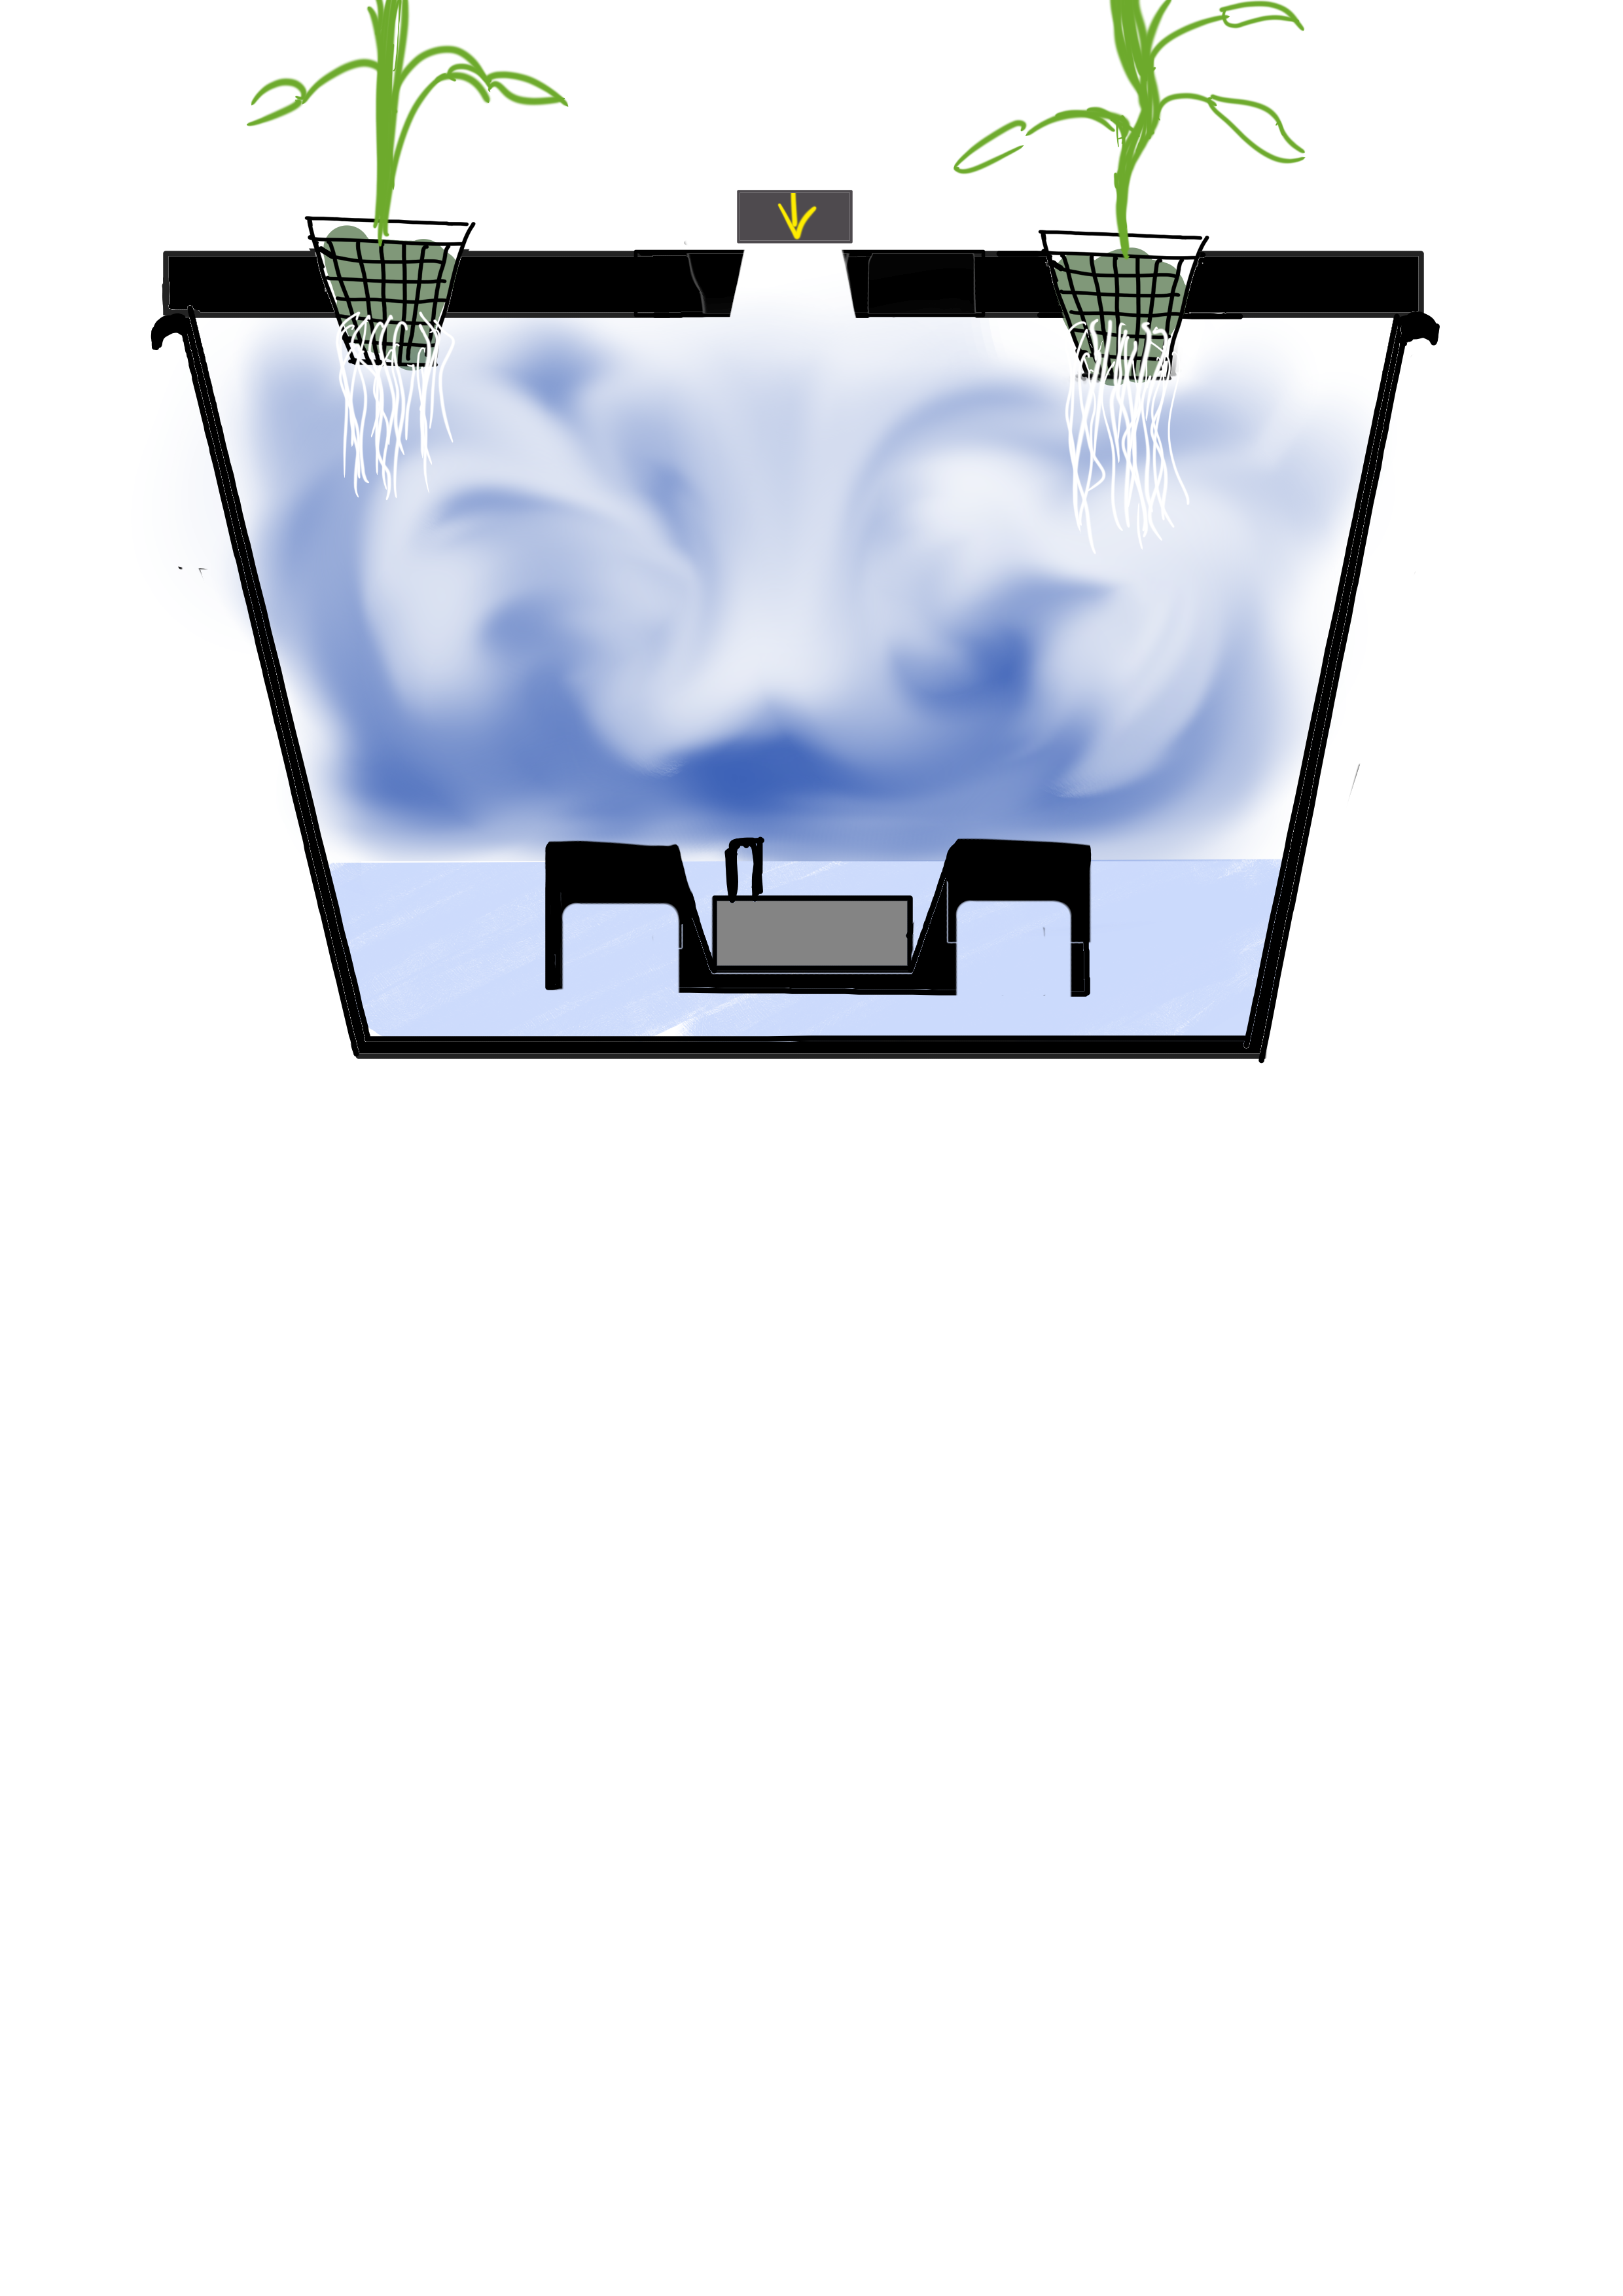
\includegraphics[width=8cm]{Querschnitt}
Ich zweckentfremde  bei beiden das mittlere Loch und setze einfach das Lüfterchen drauf. In einem meiner \textit{Forschungsaufbauten}, ich das vorhin kurz erwähnt, fand ich heraus, dass 35\% PWM für das Lüfterchen genau im perfekt Nähnebelpegel resultiert. Das einzige Problem ist jedoch folgendes: Beim PWM-Controller-Arduino brachte ich es nicht hin, für vier Pins, weil es ja vier Lüfter hat, jeweils einen eignen \textit{TimerOne}-PWM-Timer zu stellen. In meinem Fall haben nur Pin 9 und 10 miteinander funktioniert. Das alleine für vier Lüfter reicht nicht, ich brauchte noch mindestens einen mehr. Ich habe also die eingebaute PWM-Funktion, mit 1kHz hinzugenommen. Und zwar auf Pin 3, von dort aus wird zurzeit das kleine Lüfterchen gesteuert. Die geringe Frequenz führt unter anderem dazu, dass es lauter summt und quietscht als bei den vierzigfachen Frequenzen der Pins 9 und 10. Auf Pin 10 ist der Turbulenzlüfter angeschalten und auf Pin 9 \textit{zwei} Lüfter, welche die Zentrallüftung übernehmen, einer oben in der Growbox und einer unten. Das Quietschen beim Lüfterchen kommt höchstwahrscheinlich vom Stocken, also dem Motor, der noch recht gut zwischen An und Aus unterscheiden kann. Das führt zu Vibrationen, welche sich gut im Holz ausbreiten. Das möchte ich jedoch nicht, denn mein Schlaf ist mir heilig. Was ich also tat, war es, die Lüfterchenvibrationen einfach mit Watte und \textit{Ducttape} abzufangen, dadurch wurde es schon viel besser.


\subsubsection{Klick, klick}
Die LEDs mit ihrem \textit{18h zu 6h-Rhythmus} könnte ich noch fast von Hand abschalten, wenn ich ins Bette gehe und wenn ich wieder aufstehe. Doch den Fogger, den kann ich nicht alle 20s einschalten und ihn nach 10 wieder ausmachen. Das wär mir zu blöde und das würde das Ziel dieses Projekts verfehlen, das Giessen muss ja eben automatisch geschehen. Den Relay-Controller habe ich genau für das konstruiert. Einstecken, online den Rhythmus eingeben und einfach sein lassen. \textit{Set-and-Forget} ist hier das Motto. Das funktioniert sehr gut. Doch Sie fragen sich vielleicht \textit{wie}. Nachdem ich den complettenk Relay-Timer-Code von Arduino/C++ auf Python übersetzt hatte, habe ich ihn verworfen und einen neuen Ansatz verfolgt. Es ist vielleicht gut zu wissen, dass es ganz grob zwei Arten gibt, mit welchen man an dieses Problem herangehen kann. Die erste liegt darin, sich für jedes der vier Relays einen Timer zu stellen, der individuell abläuft. Ist er abgelaufen stellt man sich einen neuen Timer und sendet ein Flip-Signal an den Relay-Controller. Dieser weiss was er damit zu tun hat und schaltet das gewünschte Relay um. Die zwei verwendeten Zeiten sind die \textit{offtime} und die \textit{ontime}, welche man in Sekunden definiert. Zusätzlich hat gibt es noch den \textit{starttimer}, welcher einfach, wenn er nicht 0 beträgt, am Anfang abgewartet wird. Somit kann ich sichergehen, dass der Lichtzyklus erst am Morgen anfängt und nicht zum Zeitpunkt, an dem man es im Interface eingibt. Diese Variante birgt den Nachteil dass sie besonders schlecht mit Änderungen an den Werten klarkommt, wenn der Timer erst mal läuft. Man könnte den laufenden Timer natürlich einfach abwarten lassen, doch bei 18h macht das keinen Sinn. Der andere Ansatz ist das 1-Sekunden-Verfahren. Es ist eine bei weitem nicht perfekte Lösung und ein richtiger Informatiker mag sie auf als \textit{dirty} bezeichnen, doch sie funktioniert und das ist die Sache, die unter Zeitstress zählt. Anstatt volle 6h oder 20s oder 10s oder 18h abzuwarten, wartet man einfach immer nur eine Sekunde, danach zieht man eine Sekunde vom Timer ab. Wenn der Timer auf 0 steht, wechselt man einfach, sendet also wie vorher beschrieben das Flip-Signal und macht stellt den Timer, auf die \textit{ontime}, wenn es vorher die \textit{offtime} und umgekehrt wenn nicht. Hier ist der Code der \verb&relays.py&-Datei
\begin{lstlisting}[language=Python]
from daemon import relays

def update_rl_arr(ID):
	timer = 0
	ontime = 1
	offtime = 2
	state = 3
	#expecting a list as input with the 
	#following format: [timer, ontime, offtime, state]
	relays[str(ID)][timer] = relays[str(ID)][timer] - 1	
	if relays[str(ID)][timer] < 1:
		relays[str(ID)][timer] = relays[str(ID)][ontime] if relays[str(ID)][state] == "off" else relay[str(ID)][offtime] 
																			# set timer to ontime if the old state was "off"
		relays[str(ID)][state] = "off" if relays[str(ID)][3] == "on" else "on" 				#set state to off if it was on, else on
		send_flip_token(ID)

def send_flip_token(serial_object,ID):
	serial_object.write(ID.encode())
\end{lstlisting}
Der Import ganz oben macht das \verb^relays^-Objekt für den Code in dieser Datei zugänglich. Dieses Objekt ist ein sogenanntes Dictionary. Diese Datenstruktur funktioniert mit dem \textit{Key - Content}-Prinzip. für einen bestimmten  \verb^key^ habe ich gewissen \verb^content^, in diesem Fall ist es eine Liste mit Werte, drei Zahlenwerte und ein Wort. Die Funktion  \verb^update_rl_arr^, was soviel wie \textit{update-relay-array} heisst, wird nach jeder Sekunde einmal aufgerufen und subtrahiert 1 vom  \verb^timer^. Der \verb^timer^ steht an der ersten Stelle der Liste/des Arrays. Diese List stellt den Content dar, welche man mit dem  \verb^key^, in diesem Fall  \verb^ID^, zugänglich macht.  \verb^ontime^ steht demnach an zweiter Stelle (man beachte, dass man bei Arrays/Listen bei 0 zu zählen beginnt),  \verb^offtime^ and dritter und  \verb^state^ an vierter. Das Format sehen sie nochmal im Kommentar auf der achten Zeile. Was ich ihnen vorher mit Worten beschrieb, findet sich hier als Python-Code. Ich benutzte mehrere Python-Finessen um den Code zu verkürzen, was es womöglich etwas komplexer macht, doch versuchen sie ihn wie einen Englischtext zu lesen. Die Funktion  \verb^send_flip_token(serial_object, ID)^ ganz am Schluss macht das, was der Name schon aussagt. Ich übergebe ihr via \verb^serial_object^ die serielle Schnittstelle und  \verb^ID^ das zu flippende Relay. Den Rest übernimmt der Relay-Controller in der kleinen, grauen Box.

\subsubsection{Die kleine, graue Box mit Steckdosen drin}
Die kleine, graue Box mit Steckdosen drin heisst auch Relay-Controller, jetzt allerdings ist von der Hardware die Rede, die Software haben gerade besprochen. Sie besteht aus einem Kunstoffquader, der auf den Seiten Gummi-Deckel hat, diese Deckel lassen sich entfernen, um Kabeln  Zugang zu bieten. Ich glaube, dass es normalerweise ebenfalls dafür benutzt wird, Stromkreise zu verbinden. Eine Platine reinzuschrauben ist wahrscheinlich aber nicht vorgesehen. 
\begin{wrapfigure}{L}{0.3\textwidth}
\centering
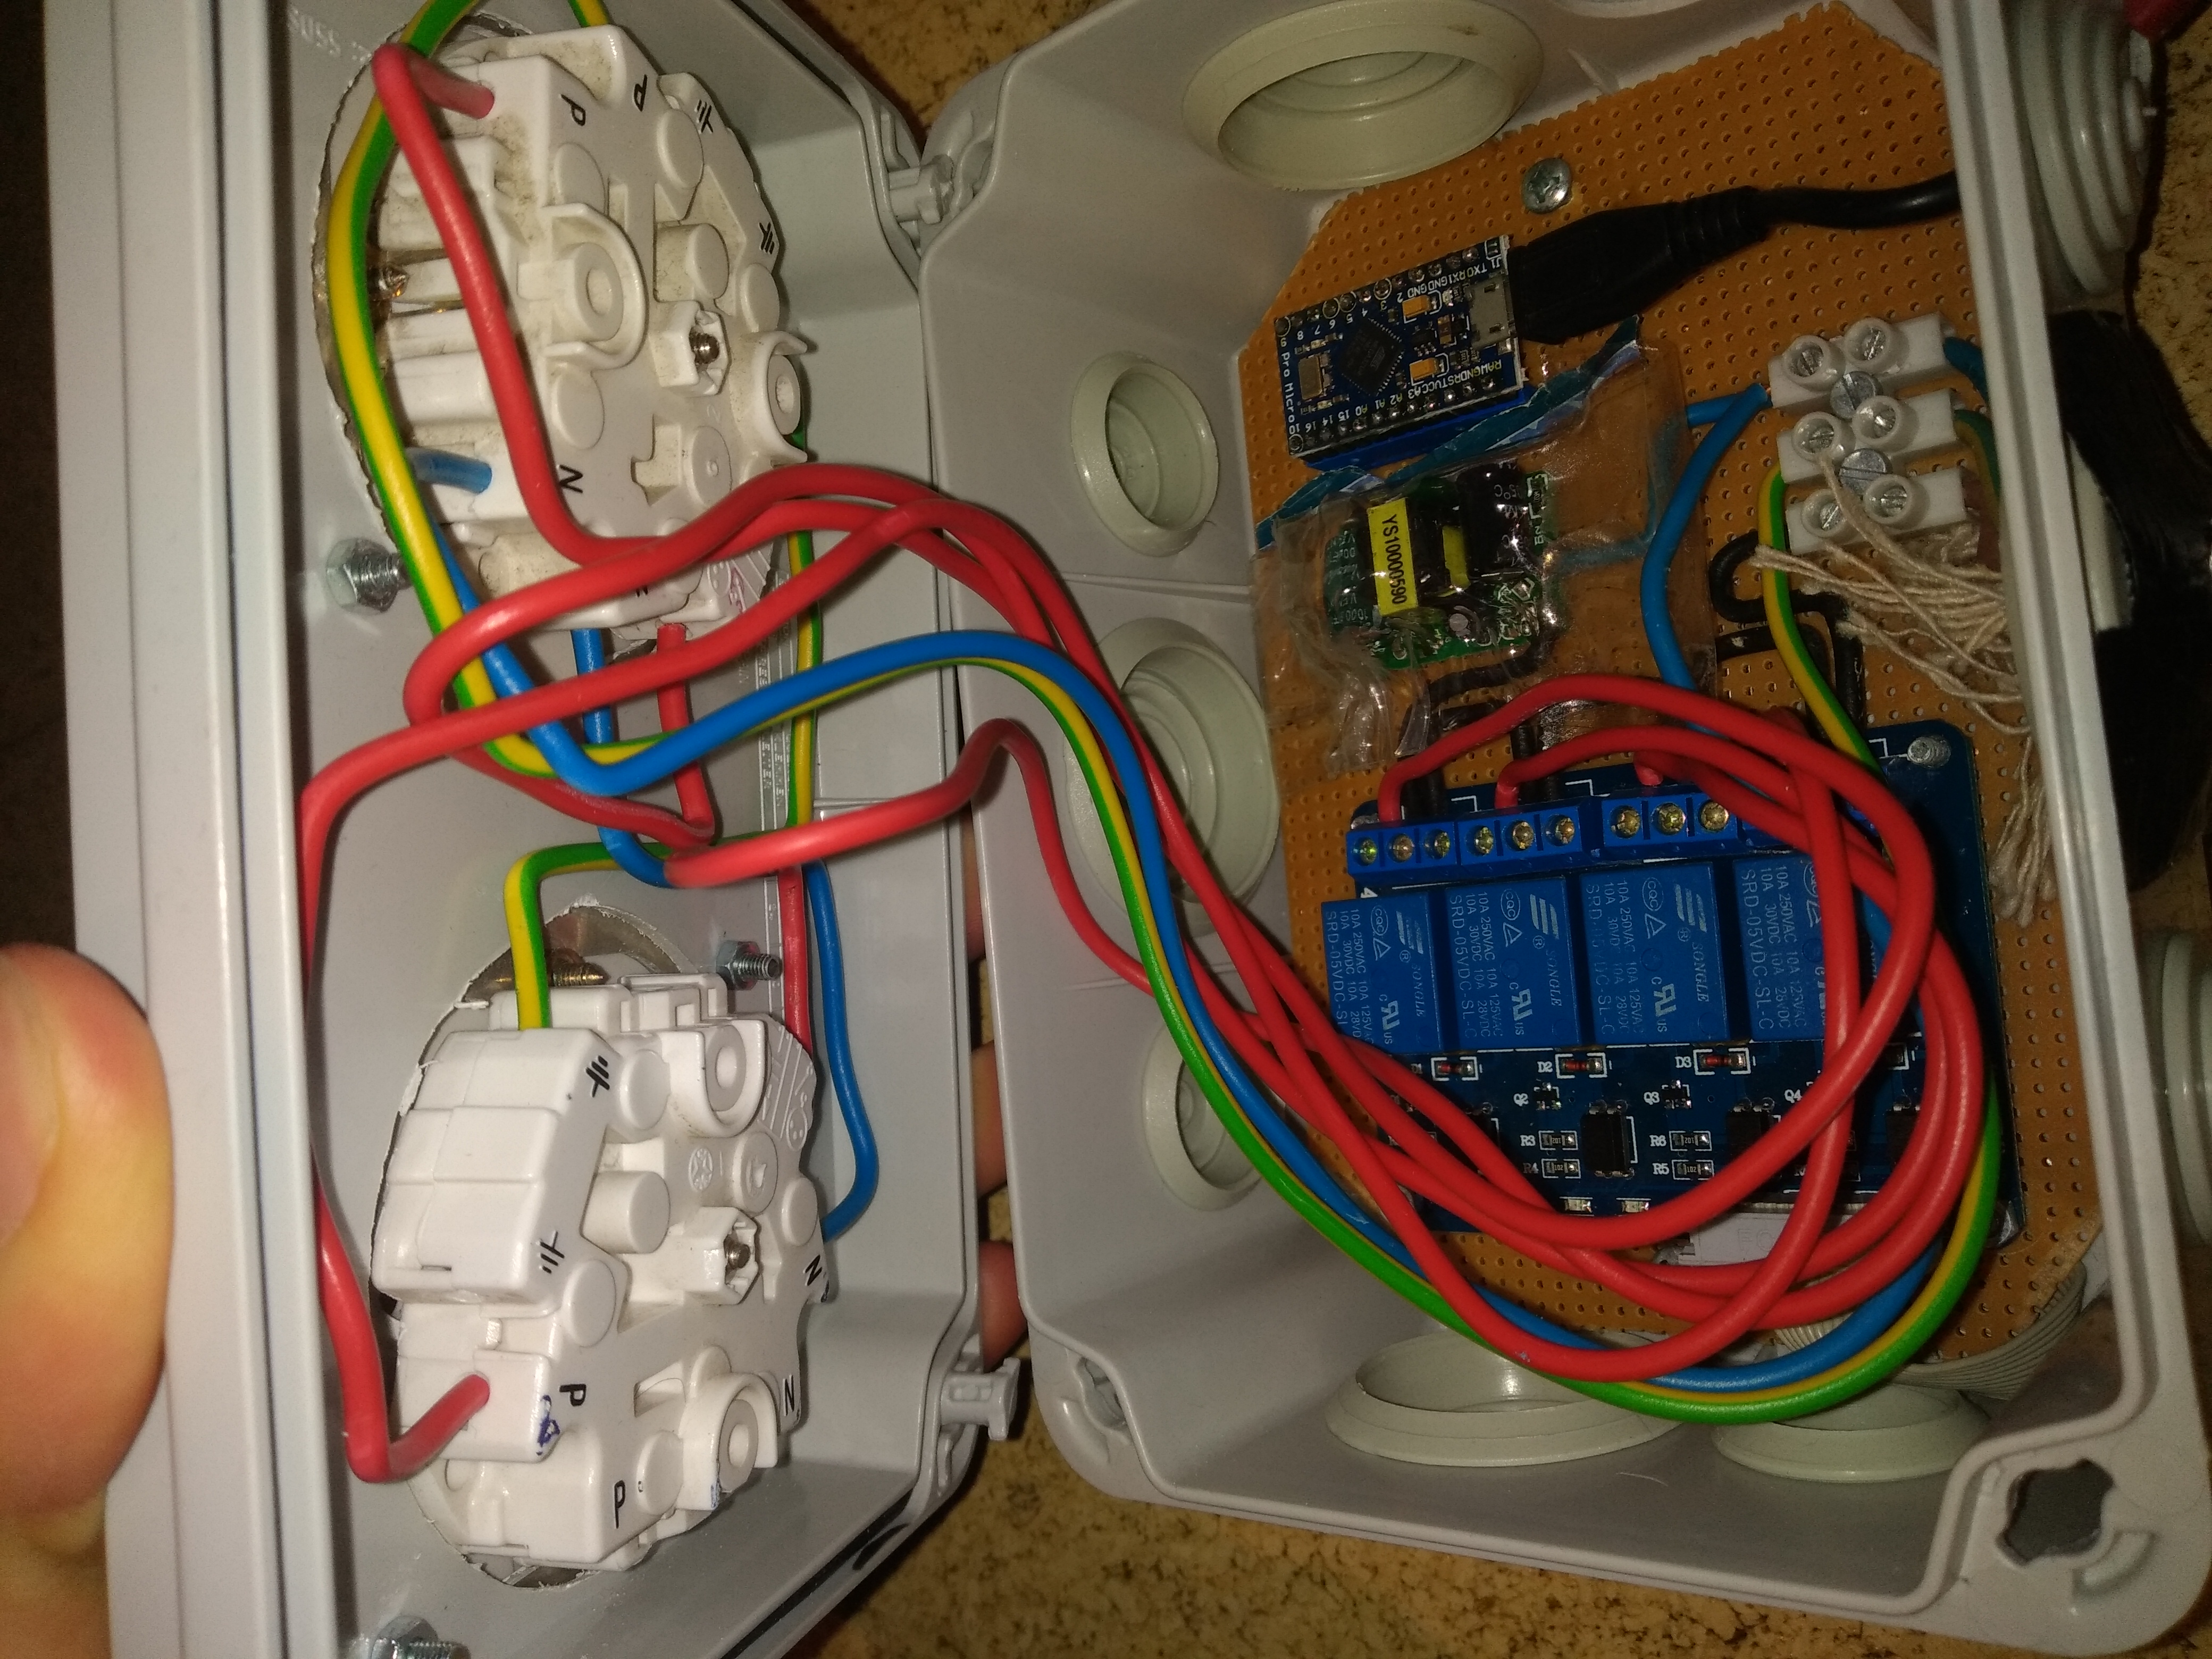
\includegraphics[width=0.4\textwidth, angle=-90]{relay}
\caption{\label{fig:relay}Der aufgeklappte Relay-Controller. Relays: links in blau. Arduino: rechts}
\end{wrapfigure}

Das ist mir egal, denn es hat die perfekt Grösse und und lässt sich sehr gut abdichten. Der abnehmbare Deckel ist mit einem Abdichtungsring versehen. Deshalb war es etwas schwer, zwei riesige Löcher reinzuboren, durch welche ich die beiden Steckdosen stecken konnte. Sie haben gerade noch so Platz, viel Freiraum bleibt nicht. Eine solche Steckdose hat drei \textit{Steckdosen}, also insgesamt hat es 9 Pins, war heisst, dass man drei schweizer Stecker damit verbinden kann. Das habe ich zweimal, was es mir erlaubt, sechs Geräte mit Strom zu versorgen. Das etwas unlogische an diesen Steckdosen ist der Fakt, dass nicht alle Steckerauffassungen (da wo \textit{ein} Stecker reingeht) einen eigenen Stromkreis besitzen, sondern dass nur eine Auffassung einen eigenen hat und sie die anderen beiden einen Stromkreis teilen. Das bedeutet, dass ich nur vier Auffassungen individuell ansteuern kann, von der Anzahl Relays passt das aber perfekt. Um den Stromfluss einer Auffassung zu unterbrechen, schalte ich einfach das dazugehörige Relay aus, welches Teil eben dessen Stromkreises ist. Diese ganze Verkabelung ist recht steif, aber ich habe genügend lange Kabel benutzt, damit ich den Deckel immer noch abnehmen kann. Die Platine, welche die Relays, den Arduino und das kleine Netzteil beherbergt ist am Boden angeschraubt, bombenfest. Es ist eine dieser \textit {einmal machen, dann aber richtig}-Lösungen, welche mir mein Vater immer eingetrichtert hat. Sie funktioniert. Daran angeschaltet sind beide LEDs und der Fogger, alles liess sich per Webinterface vorprogrammieren.

\clearpage

\subsection{Der Dämon} 
 Den Beschwörungsprozess des Dämons habe ich bereits geschildert.  Die Geisterbrücke mit \verb^rsync^, Sie erinnern sich? Jetzt geht es darum, \textit{was} ich mit Sublime genau heraufbeschwört habe. Die Aufgabe des Dämons ist es, alle Hintergrundprozesse abzuarbeiten, dazu gehören: Die Entgegennahme von neuen Werten, welche ihm der Flask-Webserver mitteilt, die Berechnung der Lüfterstärke basierend auf der Temperatur, die Mitteilung dieser PWM-Werte an den PWM-Controller und zu guter letzt der komplette Relay-Algorithmus. \\ Wenn man den Dämonen das erste Mal startet, iniziiert er die Kommunikation mit beiden seriellen Schnittstellen, also dem PWM-  und dem Relay-Controller. Ein Problem, auf welches ich schon recht früh aufmerksam wurde, war die Besorgnis, wie ich dem Dämonen mitteile, welcher Port zu welchem Controller gehört. Die USB-Schnittstellen erscheinen unter einem Linux-System mit den Namen  \verb^ttyACM0^ und \verb^ttyACM1^ im  \verb^/dev^-Verzeichnis, dort werden alle echten und virtuellen Geräte aufgelistet. Der Raspi hat einen gewissen Prioritätscheck, welchen er bei jedem Start durchführt, darauf basierende verteilt er den USB-Schnittstellen ihre Namen, entweder \verb^ttyACM0^ oder \verb^ttyACM1^. Da ich diesen Prioritätscheck erstens nicht verstehe und ihm zweitens auch nicht voll vertraue, habe ich meinen eigenen kleinen Check geschrieben, womit der Dämon, rausfinden kann, welcher Controller auf welchem Port zu erreichen ist. Um es ganz einfach auszudrücken, macht der Dämon beide Ports auf, schickt bei beiden das Signal  \verb^99^ und weiss anhand der Antworten, wo welcher Controller angeschlossen ist. Die Controller sind natürlich darauf programmiert, bei sich einem eingehenden  \verb^99^-Signal zu identifizieren. Für diesen kleinen Algorithmus habe ich länger gebraucht, als mir lieb ist, allderdings habe ich eine Menge gelernt, vorallem in Sachen wie \textit{Serial Communication}. In meinen Logs findet man nicht nur einmal die Aussage \textit{serial com is a bitch}, denn es fühlte sich mehrmals danach an. Auf das Endprodukt dieser kleinen Spielerei bin ich allerdings recht stolz, sie ist wie jede andere Datei auf meinem GitHub-Repo zu finden, auf welches ich am Schluss noch zu sprechen komme.\\Wenn der Dämon also weiss, wo er es mit welchem Controller zu tun hat, braucht er erstmal die Startdaten, welche sich in einer Datei im gleichen Verzeichnis befinden, diese Datei nennt sich  \verb^local_properties^, es gibt auch noch eine Datei namens  \verb^remote_properties^. Der ganze Clou hinter der Kommunikation zwischen dem Dämonen und dem Webserver liegt in diesen beiden Dateien. Die beiden Dateien sollen immer möglichst auf dem gleichen Stand sein. Mit \verb^remote_properties^ speichere ich jedesmal eine Änderung der Werte, wenn ich etwas im Interface verändere, zum Beispiel, wenn ich die Standart-PWM-Stärke für die Lüftung von 40 auf 50\% anhebe. Der Webserver aktualisiert den Wert einfach in \verb^remote_properties^ mit einer recht genialen Funktion, welche sich \verb^update_prop_or_relay^ nennt.
 \begin{verbatim}
 #key can be just a key for properties or the id for relays
def update_prop_or_relay(key, newvalue, path=REMOTE_PROPERTIES):
	print(f"updating {key} in {path}")
	properties = {}
	relays = {}
	with open(path, "r") as f:
		for line in f.readlines():
			values = line.split()
			if values[0] == "relay":
				if values[1] == key: #check if i can already overwrite the old stuff
					relays[key] = newvalue #as we expect to change a relay, "newvalue" should be a list.
				else:
					relays[values[1]] = [values[2], values[3], values[4], values[5]] # if it didn't match, write the normal values instead 
			elif values[0] == key:
				properties[key] = newvalue #and if it wasn't a relay, just save it as a property. Here it doesn't need to be a list.
			else:
				properties[values[0]] = values[1]
	save_props_and_relays(relays, properties, path)	#save them all
 \end{verbatim}
Alles was sie macht, ist, dass sie die bestehende \verb^remote_properties^ als funktionseigene Dictionaries, \verb^relay^ und \verb^properties^ speichert und den zu verändernden Wert direkt auf den neuen aktualisiert. Anschliessend speichert sie alles wieder mit  \verb^save_props_and_relays()^. Wenn in einem Dateiensystem eine Datei verändert wird, ändert sich auch ihr \verb^last modified timestamp^, also der Zeitpunkt, an dem man sie das letze mal änderte. Der Dämon merkt das und weiss dann sofort, dass sich etwas verändert haben muss. Was macht er also? Er synchronisiert \verb^remote_properties^ mit \verb^local_properties^ und hat somit eine Kopie von \verb^remote_properties^ zur Hand, aus welcher er die Werte ausliest, um mit ihnen weiterzumachen. Alle werte in diesen beiden Dateien sind diese:
\begin{verbatim}
relay 1 0 10 20 off
relay 2 0 64800 21600  off
relay 3 0 64800 21600  off
relay 4 0 64800 21600  off
opt_temp 24
max_delta_t 3
std_pwm 40
vent_mode auto
pwm_vent 40
pwm_fog 35
pwm_turb 50
\end{verbatim}
Relay 1 und 2 sollten selbsterklärend sein. 3 und 4 werden nicht gebraucht, deshalb ist es egal, welche Werte sie besitzen, aus ästhethischen Gründen gebe ich einfach die Werte der Lampe mit. Wenn sie auf 0 stehen würden, würden sie jeden Zyklus umschalten, was einen Höllenlärm verursacht. Wenn sie aber ebenfalls im 18h-6h-Zyklus der Lampe laufen, ist mir das recht. \verb^opt_temp^ ist die Optimaltemperatur, \verb^max_delta_t^ die Temperaturdifferenz zwischen der 100\%-PWM-Grenze und der Optimaltempereatur, \verb^std_pwm^ die Standart-PWM-Stärke für die Lüftung (damit der C0$ _{2} $-Austausch gewährleistet ist), \verb^vent_mode^ ist entweder \verb^auto^ oder \verb^manual^, je nachdem ob man die Lüftungstärke automatisch anpassen möchte, \verb^pwm_vent^ ist die Lüftungsstärke, dieser Wert wird automatisch berechnet, wenn \verb^vent_mode^ gleich \verb^auto^ ist, \verb^pwm_fog^ ist die Lüfterchenstärke für die Nährnebelturbulenzen und \verb^pwm_turb^ schliesslich die Stärke für den Turbulenzventilator.\\ \\Mit diesen Werten arbeitet der Dämon jede Sekunde, er schaut ob sich was verändert hat, wenn ja, synchronisiert er sie, liest sie ein und macht dann weiter. Diese Aktion läuft in einer Endlosschlaufe und hört erst auf, wenn ich den Prozess abschiesse.

\subsection{Den Code selbst lesen}
Wenn Sie den Code selbst lesen oder weiterentwickeln wollen lade ich Sie natürlich herzlichst dazu ein. Sie finden ihn auf https://github.com/schnippo/ssgb



\subsection{Ungenauigkeiten}
Welche Annahmen in meiner Maturarbeiten sind ungenau? Ich habe dieses Thema schon kurz bei der Lüftungssteuerung angeschnitten. Ich möchte hier aber dennoch noch kurz auflisten, welchen Werten ich nicht vertraue, respektive in welchen Bereichen ich aus dem Bauchgefühl handelte. Dies ist zwar eine gestalterische Arbeit, jedoch setzt sie sich mit einem wissenschaftlichem Thema, der Lebenserhaltung von Pflanzen, auseinander. Aus diesem Grund möchte ich dem wissenschaftlichen Teil mindestens dadurch Genüge leisten, indem ich Bereiche der Ungenauigkeit aufzähle.\\ Als allererstes könnte ich mich beim CO$ _{2} $-Verbrauch der Pflanzen komplett irren, ich habe mir schlicht die Mühe nicht gemacht, diesen Aspekt zu behandeln, obwohl ich dies im Nachhinein bereue, denn es hätte gut in die Arbeit gepasst und mir mehr Sicherheit verschafft. Dass ich es bis jetzt nicht gemacht habe heisst allerdings überhaupt nicht, dass es \textit{nie} geschehen wird. Die Abgabe dieses schriftlichen Einblicks in mein, ich würde es nicht \textit{Lebens}projekt nennen, aber es geht in diese Richtung, in mein Projekt ist nur ein kleiner Punkt auf dem Zeitstrahl. Wenn Sie sich also wundern, wie ich an diese Fragestellung herangehe: Ich verspreche Ihnen, das README.md, also die Startseite der GitHub-Seite so zu aktualisieren, dass es ersichtlich ist, wenn ich den CO$ _{2} $-Verbrauch berücksichtige.\\ Weitere Annahmewerte waren alle Temperatur- und Feuchtigkeitswerte. Proteine denataurieren ab etwa 35° Grad, bis unter diesen Wert funktioniert die Photosythese immer schneller. Rein theorethisch liegt es also in meinem Interesse, den Pflanzen genügedn CO$ _{2} $ zu liefern, während ich die Temperatur möglichst hoch halte, aber unter 35°. Schon während ich das hier schreibe, kommt mir die Idee für eine neue Art Thermostat. Er wird wohl aber noch etwas warten müssen. Einer rein wissenschaftlichen Arbeit täte ich mit solch gravierenden Ungenauigkeiten kaum Genügen. Aber das ist eine gestalterische Arbeit und es geht um die Erfolge wie Fehler des Konstruktionsprozesses.



\section{Perspektiven}
In diesem Kapitel mache ich Sie mit harten Einsichten, erlernten Fähigkeiten und neuen Perspektiven bekannt.

Einhergehend mit den Arbeitsprozessen, bekam ich auch neue, mir zuvor völlig undenkbare Einsichten und Perspektiven 
\subsection{Technisches Upgrade}
Es ist komplett offensichtlich, dass ich eine ganze Menge über Technik gelernt habe. Im Kapitel \textit{Arbeitsprozess} bin ich darauf eingegangen was ich wie gemacht habe. Jetzt zeige ich Ihnen auch noch, \textit{was} ich daraus gelernt habe. Ich kann Ihnen natürlich nicht einfach sagen dass ich gelernt habe, dass z.B. Dioden Strom nur in eine Richtung durchlassen, denn das ist selbst für mich etwas langweilig. Ich erwähne deshalb nur den groben Teilbereich, mache ein, zwei \textit{spannende} Beispiele und gehe dann zum Nächsten.
\subsubsection{Oszilloskop und Elektronik}
Ich habe es bereits gelobt. Eine Wundermaschine mit der ich mein Verständnis fürs Verhalten von elektrischem Strom verbessern konnte. Um in meinem Beispiel ein PWM-Signal zu visualisieren, muss man den Strom durch \textit{den Fühler} leiten, so nenne ich es. Der Fühler hat zwei Klemmen, eine kommt an die Masse-/Minusleitung und der andere an entweder die Basis oder den Emittor des Transistors. Den Transistor erkläre ich auch nur kurz: Er hat drei Pins, Basis, Emittor und Kollektor. Vereinfacht geht der Strom beim Kollektor rein, und verlässt ihn mit einer um, einen Transistor-spezifischen, Faktor verstärkten Spannung beim Emittor, aber \textit{nur} wenn bei der Basis eine Minimalspannung von 0.7V angelegt wird. Es funktioniert also im Grunde wie ein Relay, einfach mit Spannungsverstärkung. Das Oszilloskop habe ich oft gebraucht. Es hat vier \textit{Fühler}, wovon aber maximal zwei nötig waren. Die Darstellung des Signals, also Frequenz, Amplitude und Grundwert lassen sich alle entweder manuell oder automatisch einstellen. Man kann auch gewisse Triggerpoints setzen, welche das Oszi dazu bringen, nur Werte anzuzeigen, welche diesen Trigger erreichen.

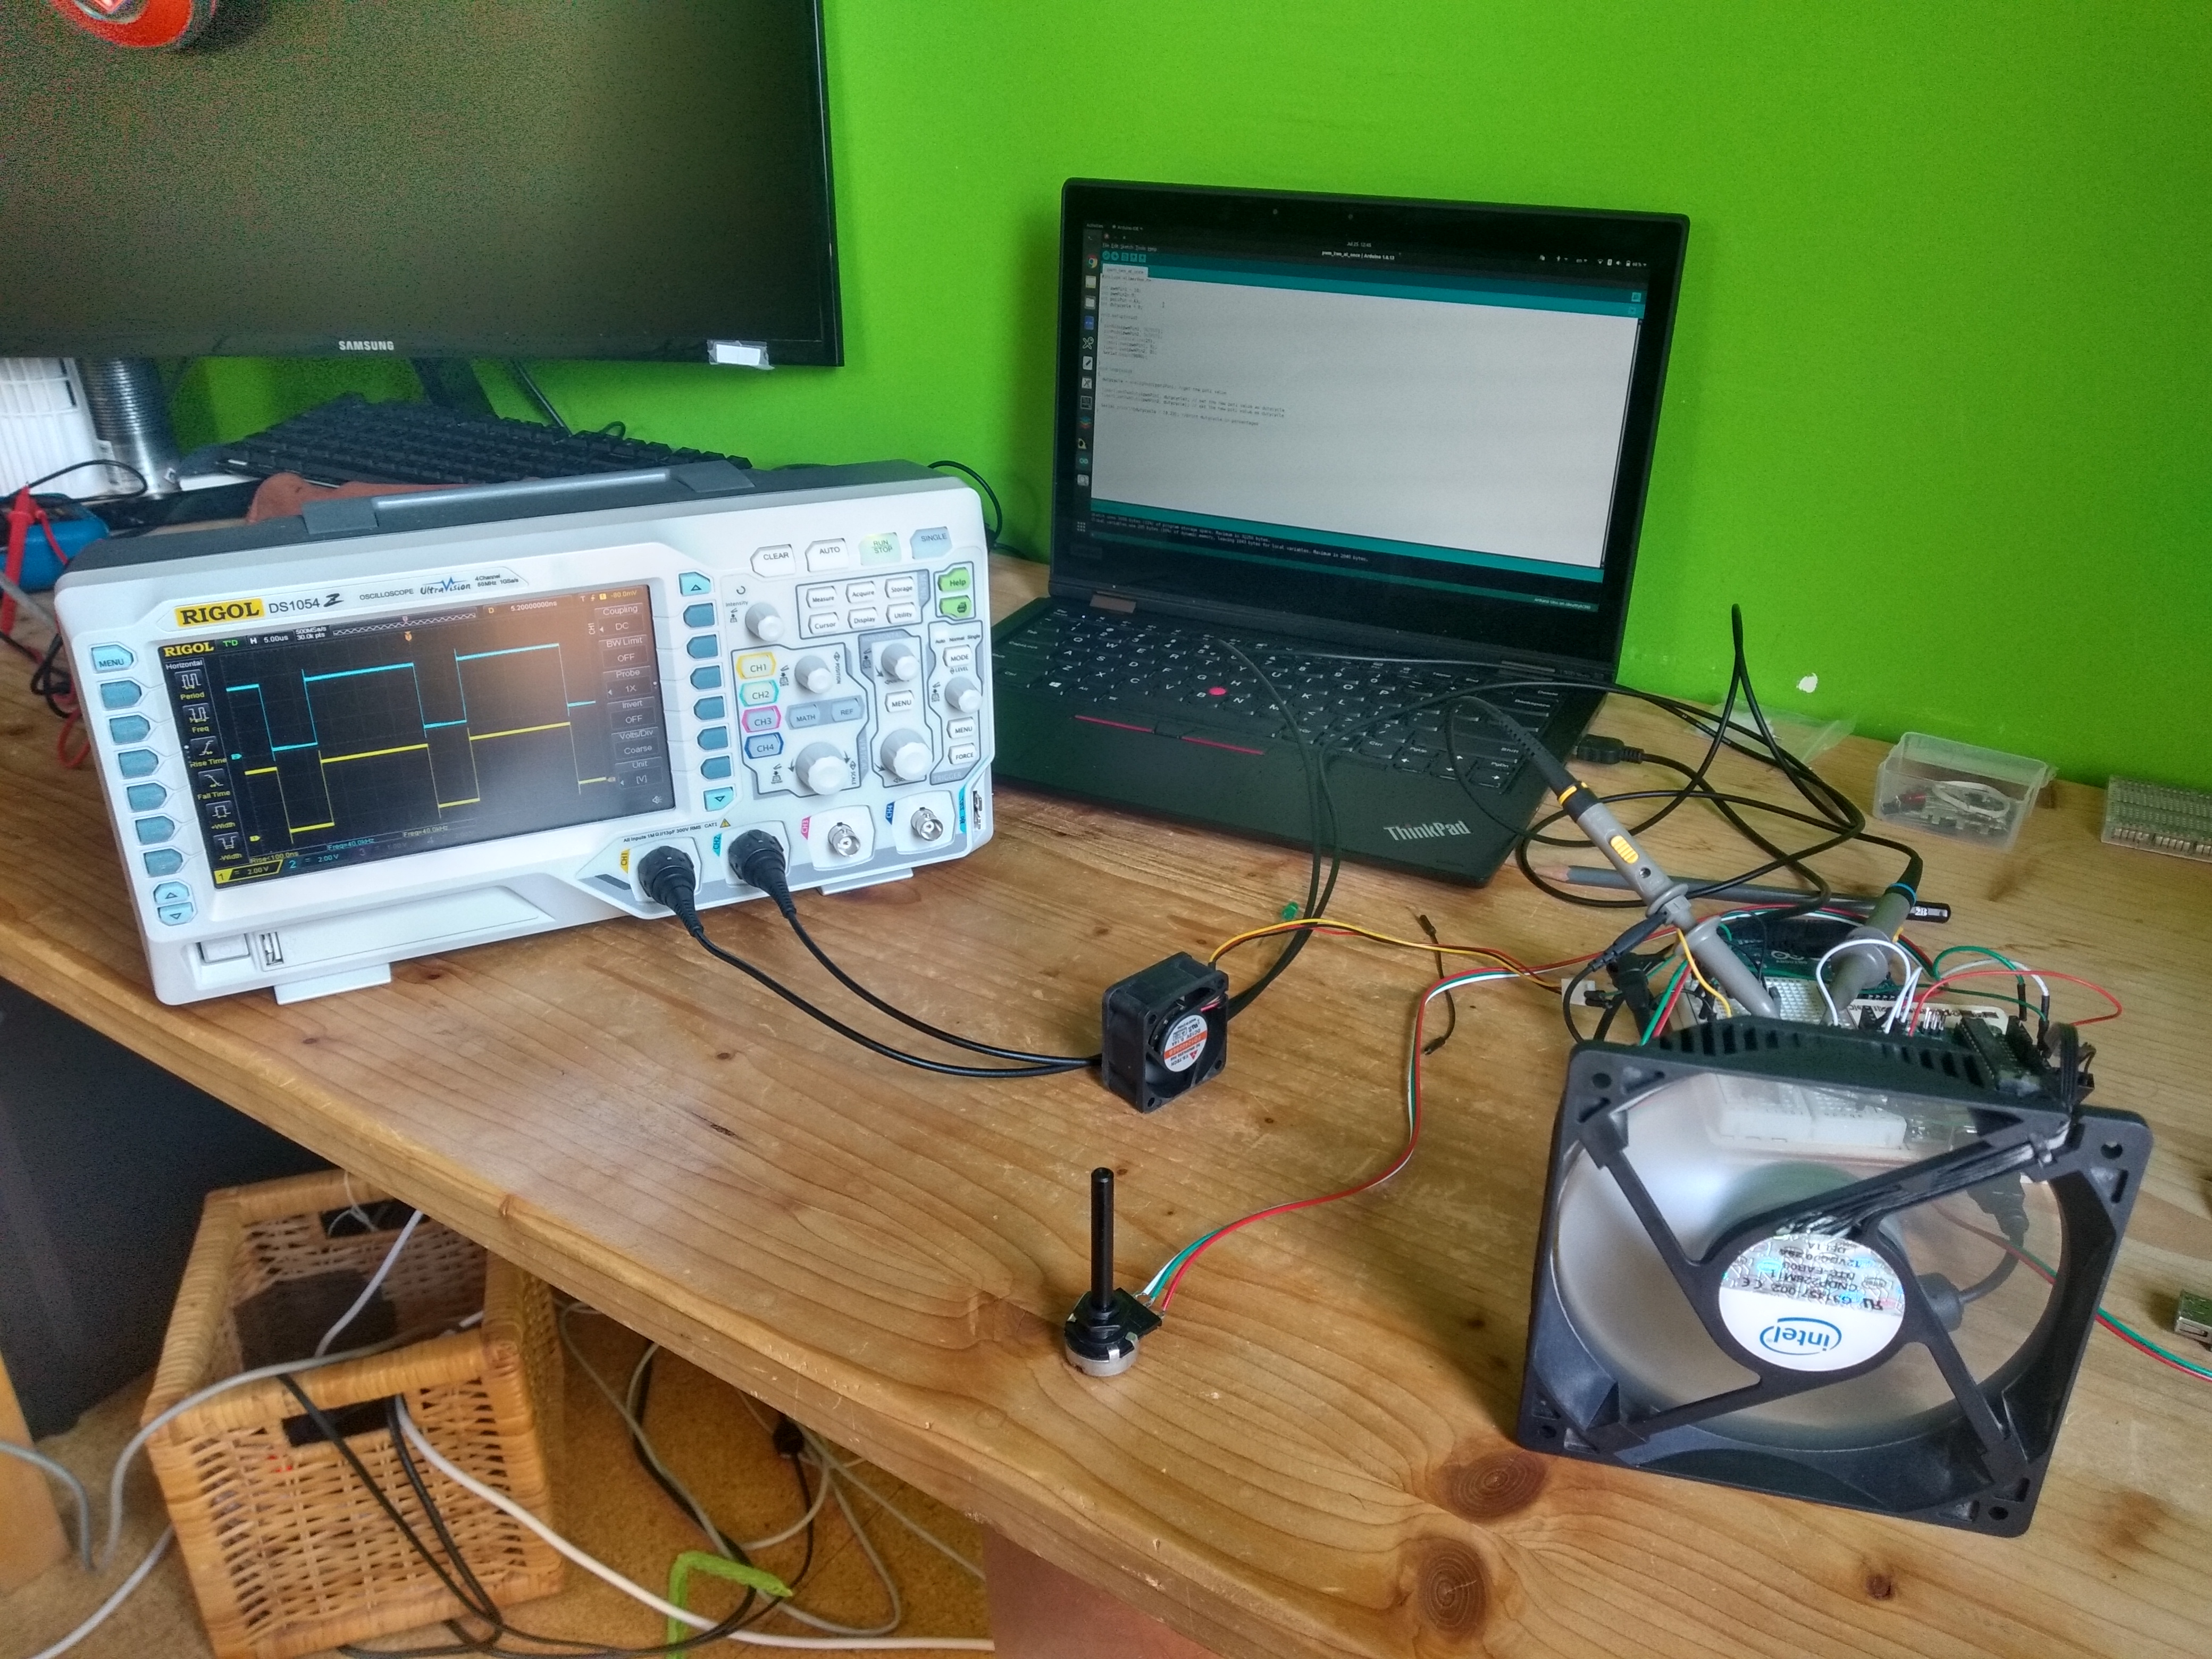
\includegraphics[scale=0.07]{oszi2}
Nach ein paar Abenden hatte ich den Dreh recht gut draussen.\\Was ich auch zu schätzen gelernt habe sind Schaltpläne. Ohne Schaltplan hat sich mein Vater geweigert, eine Schaltung auch nur anzusehen. Ich kann es ihm nicht verübeln, denn es macht einfach keinen Sinn, planlos irgendwelche Sachen zu messen. Man baut ohne Bauplan ja auch kein Haus. Einen Schaltplan zu zeichnen ist guter Spass und schafft Klarheit. Die Software \textit{Fritzing } erlaubt es einem sogar, echte Module wie einen Arduino für seinen Plan zu benutzen. Ich habe das ein- oder zweimal gemacht, es sah schön aus aber mit einem Bleistift und etwas Kritzelpapier ist man schneller und ausserdem auch noch authentischer.\\Meine Lötskills habe sich ebenfalls um einiges verbessert, das wurde bereits klar. Viel kann ich dazu nicht sagen, man sollte darauf achten, dass der Lötkolben immer etwas Zinn dran hat, aber nicht zu viel. Ausserdem verzinnt ein richtiger Elektroniker zwei Kabel immer, bevor er sie zusammenlötet. Das Leben kann sehr einfach sein, wenn man nur weiss wie richtig gelötet wird - das habe ich gelernt.

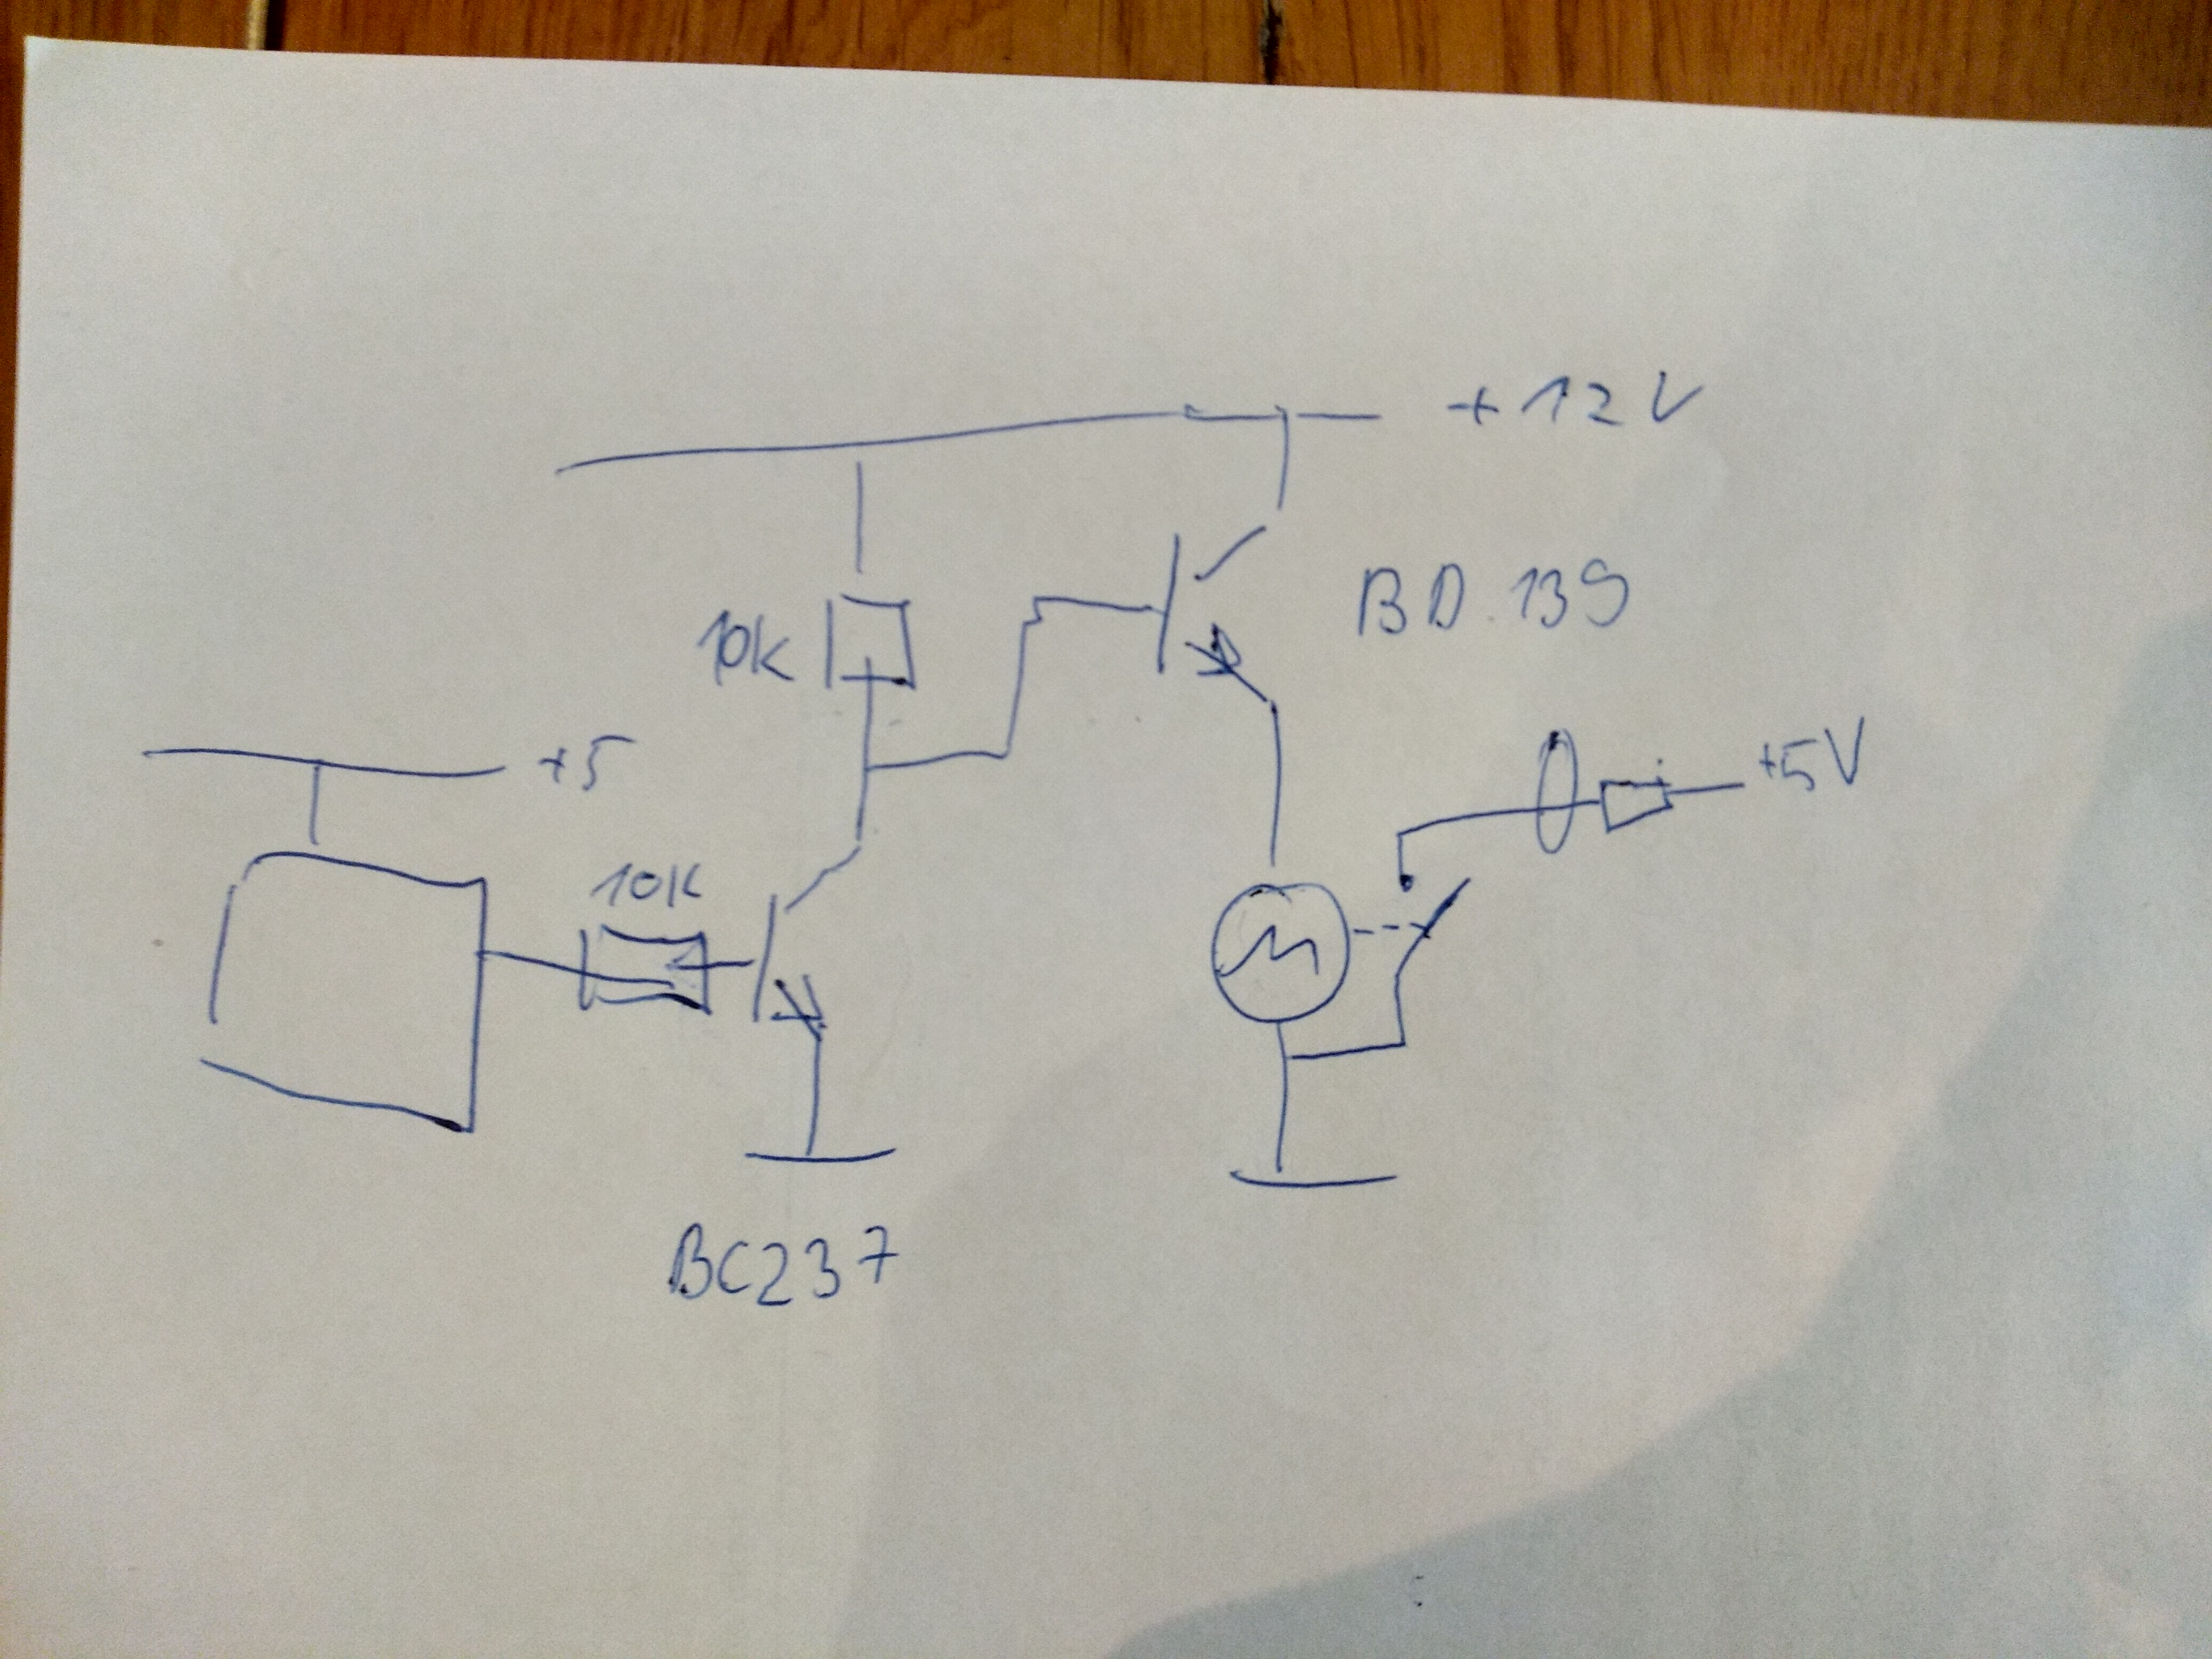
\includegraphics[width=\textwidth, angle=0]{schaltplan}

\subsubsection{Python und Flask}
Meine Begeisterung für Python war schon vorher da. Der simple Syntax und die unglaubliche Vielfalt dieser Sprache sind ansteckend. Als ich dann nach meiner C++/Arduino-Oddyssey an Land stieg und nach Hause in meine Python-Domäne ging, um den Dämonen zu beschwören, fühlte ich mich um einges wohler. Den Syntax von Python beherschte ich schon, hatte ja schon ein paar kleinere Projekte damit verfolgt, aber was mich dann so richtig überzeugte, waren die Oneliner - \textit{Ternary Expressions}. Sie sind die einzeilige Alternative zu einem vierzeiligen \verb&If - Else& wenn es darum geht, Variabeln zuzuordnen. Der Flow der damit in eine Funktion kommt ist schön anzuschauen. Es wird auf der einen Seite komplexer, da mehr Code in weniger Zeilen steht, aber gleichzeitig räumt es auch auf - Wenn man schon drei \verb&If - Else&-Statements tief in der Funktion noch ein viertes beschwört, nur um einer Variabel einen neuen Wert zu verpassen, dann lässt man sich gerne auf den Einzeiler in Form einer \textit{Ternary Expression} ein.\\Ein weiterer Stern am Pythonhimmel ist selbstverständlich Flask. Die traditionelle Webseite wird durch \verb&apache2& oder \verb&nginx& zugänglich gemacht. Das Backend, in meinem Fall also der Teil, welcher dem Dämonen das Essen serviert, wird traditionell von der \textit{PHP-Engine} dargestellt. Da ich aber noch keine einzige Zeile PHP-Code geschrieben habe, erscheint mir eine Alternative wie Flask wahrhaftig wie ein Stern am Himmelszelt. Das Framework ist mit vertretbarem Aufwand zu verstehen, jedenfalls mit \textit{Corey Schafers} YouTube-Tutorial. Innerhalb weniger Tage war die Webseite auf meine Bedürfnisse angepasst. Ich habe eine gute Menge HTML gelernt, ein kleines bisschen CSS (wirklich nur ein bisschen; CSS gleicht dem Marianengraben) und Webprotokolle wie GET und POST sind mir nun auch nicht mehr ganz fremd.

\subsubsection{Bash und so}
Mein Frack wurde durchaus ein klein wenig länger. Entschuldigung, Pinguin- also Linuxslang: Ich habe durchaus gewisse Sachen mit der Bash gelernt. Ich gehe nicht auf alles einzeln ein, deshalb hier eine Liste der Tools, von denen ich jetzt weniger Angst habe: SSH-Keys, \verb&git&, \verb&rsync&, \verb&nohup&, \verb&stderr& und \verb&stdout&. Die Liste ist wohl länger, aber die Bash ist so riesig, dass ich mich leicht verlieren könnte.



\subsection{Signifikanz}
Das richtige Abwägen, ob eine bestimmte Funktion vom \textit{Konstrukt} ausgeführt werden können soll, ist eine Angelegenheit für sich. \textit{Decisionmaking} ist anspruchsvoll und entscheidet darüber, wieviel man arbeiten muss. Die durchführbarkeit eines Teilprojekts spielt wohl die grösste Rolle. Hier sind ein paar Beispiele.
\subsubsection{Bewässerung mit Düsen}
Davon war die Rede im Kapitel \textit{An die Arbeit}, es war zu diesem Zeitpunkt die mir einzig effizient erscheinende Option. Düsenbewässerung zählt sich zur Aerponik, welche den Ruf einer sehr effizienten und wassersparenden Bewässerungsmethode hat. Effizienz und der ökologische Fussabdruck sind beides Sachen, welche bei der Konstruktion berücksichtigen wollte. Von Fogponics war ich zuerst nicht angetan und zwar wegen dem nächsten aufgeführten Thema. Ich hatte mich falsch informiert und berechnete die Leistung eines Foggers auf mehr als 400W, was, wie Sie gleich erfahren werden, nicht tragbar gewesen wäre.

\subsection{Solar overkill}
Das Projekt heisst auf dem Maturarbeitsvertrag \textit{Automatische Vertical Gardening Anlage}. Später kam mir noch die Idee, den kompletten Stromverbrauch mit Solapanels abzudecken. Diese Idee ist unglaublich cool und es tut mir in der Seele weh, dass ich es nicht geschafft habe. In diesem Bereich habe ich versagt. Es war wahrscheinlich 70\% der ganzen Arbeitsphase geplant und ich musste mir irgendwann eingestehen, dass der Aufwand zu gross wäre. Geplant hatte ich eine eigene Solaranlage auf meinem Dach. Ich habe die Sonneinstrahlung berücksichtigt, mich im Web schlau gemacht, Preise und Produkte rausgesucht und - wie vorhin schon angedeutet - meinen gesamten Energieverbrauch zu berechnen versucht. Ich wollte also den Stromverbrauch der Lampen, des Foggers, der Lüfter und der Steuerungstechnik berechnen, damit ich wusste, wieviel Panels ich bestellen müsste und wieviel Stromspeicherkapazität es bedurfte. Dazu kamen auch Überlegungen wie schlechtes Wetter, Einstrahlungswinkel und daraus resultierend der \textit{Energiesparmodus}: Wenn die Stromreserven in den Batterien zur neige gingten, wollte ich die Leistung der LEDs runterdrosseln, damit die wirklich wichtigen Lebenserhaltungssysteme wie Bewässerung und CO$ _{2} $-Versorgung noch genung Strom hatten, um die Pflanzen bis zum nächsten Auftanken, in Form besseren Wetters oder Sonnenaufgang, durchzubringen. Der Solaraspekt meines Projekts fand seine Präsenz sogar im Titel: SSGB - Smart \textit{solar} GrowBox. So heisst das Projekt auch auf GitHub. Dass ich dem nicht nachgekommen bin und dass mein GitHub-Titel lügt wurmt mich erhlich gesagt. Rein vom Arbeitsaufwand wäre es \textit{vielleicht} schaffbar gewesen, aber meine Erfahrung ist in zu vielen Bereichen, und dieses Projekt schneidet \textit{einige} Bereiche an, einfach zu wenig gewesen. Angenommen ich hätte schonmal mit Pulsweitenmodulation gearbeitet, einen Pythondämonen beschwört oder einen einen Flask-Webserver aufgesetzt, dann hätte es vielleicht besser ausgesehen. Aber auch dann wären immer noch viele Fragen offen, einige habe ich oben aufgeführt. Wie genau installiere ich eine Solaranlage auf meinem Dach? Ich hätte niemals eine Firma dafür arrangiert, denn das wäre gegen meinen MA-Kodex, der besagt, dass ich alles selber mache. Die Befestigung der Panels, sodass sie sich auch bei einem Sturm wie \textit{Sabine} nicht  aus dem Staub machen hätte ich mit meinen Kletterkünsten wahrscheinlich noch hinbekommen, doch wie sollte ich die Hauptstromleitung \textit{in} mein Zimmer bekommen? Das Fenster für immer offen zu lassen fand ich keine gute Idee und ein Loch in mein Dach zu bohren widerspricht der Natur eines Dachs. Dächer sind ja da, um dicht zu sein. Ich hätte es also abdichten müssen - wie? Meine Situation ist klar, ich habe viel geplant, es hat nicht in die Form der Maturarbeit gepasst, aber das hindert mich nicht, es dennoch einfach später zu versuchen. Vielleicht findet sich auf meinem Git-Repo bald ein Ordner mit dem Namen \verb/solar/.

\subsection{Mögliche Weltverbesserung}
Ich habe nebst der Segel-Vision noch eine weitere Perspektive kennengelernt. Während der Recherche interessierte ich mich besonders für Vertical-Gardening-Anlagen. Ich habe zwei schweizer Unternehmen angeschrieben, ob sie mir wohl ein paar Fragen beantworten könnten oder ob ich mal reinschauen dürfte. Sie haben leider nie zurückgeschrieben und ich habe es vergessen. An sich ist das schade, denn der Rucksack mit meinen Fragen wäre bestimmt etwas leichter geworden. Es war zurzeit des Lockdowns, als alle in Panik gerieten und sich das Unternehmertum schleunigst gute Konzepte überlegte. Deshalb nehme ich an, dass beide Untenehmen zu beschäftigt waren. Meine Weltverbessererperspektive zeigt sich darin, dass ich dieses Projekt nicht nur gerne mobil (z.B. für Segelboote) sondern auch möglichst grün machen möchte. Ich träume von einem Opensource-Projekt, bei dem es nicht nur um Code, sondern auch um die Hardware geht. Wenn die Hardware möglichst umweltfreundlich hergestellt wird, wäre das ein riesen Bonus. Ich denke an recycletes Mylar für die Reflektivbeschichtung der Growbox, langlebige LEDs, und vielleicht sogar wiederverwertete Lüfter. Das wiederverten von alten Teilen habe ich selbst mit meinen Lüftern ausprobiert. Und wenn das nicht geht, denke ich mir neue Ideen und Perspektiven aus, wie sich Stadtbewohner, wenn sie möglicherweise keinen Balkon haben, trotzdem so viel Gemüse wie möglich selber anbauen könnte. Je mehr Tomaten man selbst produziert, desto weniger müssen aus Spanien eingefuhrt/eingeflogen werden. Somit kann man seinen ökologischen Fussabdruch verringern. Ich denke Sie verstehen das Konzept. Es gibt schon so viele gute Ansätze. Zum Beispiel bin ich auf das ETH-SpinOff-Projekt \textit{Yasai} gestossen. Was diese Allumnis machen, geht ganz stark in meine Richtung, mal schauen was sich daraus ergibt.



\section{Fazit}
Das Projekt war vorallem gegen das Ende hin sehr intensiv, um es schön auszudrücken. Meinen Zeitplan habe ich bei weitem nicht eingehalten, was mir aber auch nicht so wichtig ist, da die Maturarbeit nur ein kleiner Teil dieses Projekts darstellt. Raum für Verbesserung ist in vielen Bereichen noch da, das muss ich zugeben. Ich habe irrsinnig viel gelernt, meine Perspektiven haben sich verändert und ich schreite auf jedem Fall mit mehr Elan durchs Leben. Das Projekt inspiriert mich weiterhin und ich kann die Features, welche ich in den kommenden Wochen und Monaten einbauen und verbessern möchte schon gar nicht mehr an einer Hand abzählen. Die Log-Datei auf Google-Docs hat mir und ich hoffe auch meiner Betreuungsperson geholfen. Ein zentrales Element, was mir erst jetzt auffällt: Wenn ich erstmal am Arbeiten war, ging das mit der Motivation von ganz alleine, auch wenn gewissen Teilprojekte einiges an Energie kosteten - Hätte ich  mich also konstanter drangesetzt, hätte es wahrscheinlich mehr Spass gemacht. Aller Anfang ist schwer, so auch hier. Das Projekt hat so viele Interessenbereiche und \textit{Wissenschaften} vernetzt, was eine grosse Breite zur Folge hat, gleichzeitig musste ich mich auch ganz schön in die Materie knien, damit ich dem Tiefenaspekt einer solchen \textit{Konstruktion} gerecht werde; Insgesamt ist dieses Projekt sehr intensiv. In der Schule wird uns das Wissen in Form von Fächern beigebracht. Wir lernen also, in einem Fach auf eine bestimmte Weise zu denken. Dieses Projekt forderte mich aber auf, Gelerntes zu vernetzen. Denkmuster waren oft nichtmer klar voneinander zu unterscheiden, es war mehr wie ein \textit{gesamtintellektueller} Denkprozess. Diese Art von Denken ist es, was ich mir vom Gymnasium erhoffe. Das Projekt war somit Überbringer dieser \textit{finalen} Lektion. Es hat meine Entwicklung und dadurch auch meine Zukunft beeinflusst.



\section{Danke sagen}
Vielen Dank Papa für deine \textit{unendlich ansteckende} Begeisterung für die Materie der Technik. Ohne dich hätte ich dieses Projekt a) wahrcheinlich gar nicht gestartet und wenn doch b) nicht geschafft. Vielen Dank auch an Herr Kern für seine Begeisterung, auch wenn wir uns nur zweimal getroffen haben, hat mich seine Leidenschaft in Sachen Informatik inspiriert und geleitet. Das Konzept am Anfang und die klare Kommunikation haben sehr geholfen. Meine Familie und Freunde haben mich, ohne es zu bemerken, immer wieder zu neuen Überlegungen getrieben - Danke an euch alle!\\
Dem Internet möchte ich natürlich auch danken, besonders \textit{stackoverflow.com}, YouTube und natürlich den vielen 420-Shops, ihr macht einem Newcomer das Leben sehr viel einfacher.zz



\printglossary[title=Glossar, toctitle=Glossar]


%Literaturverzeichniss ins Inhaltsverzeichnis einfügen
\addcontentsline{toc}{section}{Glossar}

%\bibliography{ssgb}
\bibliographystyle{agsm}
\end{document}





